\documentclass[../main.tex]{subfiles}



\begin{document}




 \chapter{Construcció d'espais topològics}

\section{Topologies inicials i finals}

\subsection{Topologia inicial}

En el capítol (\ref{def:topologiasubespai}) hem vist com definir una topologia en un subconjunt $Y$ d'un espai topològic $X$. És a dir, induïm una topologia en $Y$ mitjançant l'aplicació $Y\hookrightarrow X$. Canviant la inclusió per una aplicació arbitrària $f:Y\rightarrow X$ es defineix la topologia
\begin{equation}
    \notag
    \tau_Y = \{f^{-1}(U)\;:\;U\text{ obert de }X\} .
\end{equation}
Aquesta topologia és la més grollera sobre $Y$ que fa contínua l'aplicació $f$. Generalitzem al cas de $n$ aplicacions.
\begin{equation}
    \notag
    f_i: Y\rightarrow X_i,\qquad i=1,\ldots, n.
\end{equation}
on $X_1,\ldots, X_n$ són espais topològics.

Així doncs, donant una definició d'aquesta topologia, la topologia inicial, podem veure que la topologia subespai és un cas particular d'aquesta topologia. Més endavant dedico un apartat sencer a explicar la topologia subespai des d'aquest punt de vista.

La qüestió és que tenim un espai topològic $Y$ i un conjunt $X$ i volem fer que la funció $f:X\rightarrow Y$ sigui contínua i construir un espai topològic a $X$ induït per $f$ (tal que sigui contínua).

\begin{defi}[Topologia inicial]
\label{def:topologiainicial}\index{Topologia inicial} Sigui $X$ un conjunt i $Y$ un espai topològic. La \textit{topologia inicial} induïda per $f$ en $X$ és la topologia més grollera a $X$ que fa l'aplicació $f:X\rightarrow Y$ contínua. En general, sigui $X$ un conjunt i $\{Y_i\;:\;i\in I\}$ una col·lecció d'espais topològics. Aleshores la topologia inicial induïda per $\{f_i\;:\;i\in I\}$ és la topologia més grollera a $X$ que fa cada aplicació $f_i:X\rightarrow Y_i$ contínua.
\end{defi}

Aleshores, prenem un conjunt $X$ i un espai topològic $Y$. Considerem $f:X\rightarrow Y$ i considerem el conjunt de tots els oberts de $Y$. Aleshores, per a que la funció $f$ sigui contínua s'ha de complir que la antiimatge de tots els oberts de $Y$ sigui obert de $X$. Per això cal dotar $X$ d'una topologia. Si el dotem de la topologia inicial, aleshores el conjunt d'oberts de $X$ és justament això: per a cada obert $V$ de $Y$ tenim $f^{-1}(V)$ com obert de $X$. Aquest seran, doncs, els únics oberts de $X$ amb la topologia inicial. No hi posarem més oberts perquè volem que sigui la més grollera possible. 

\begin{equation}
    \notag
    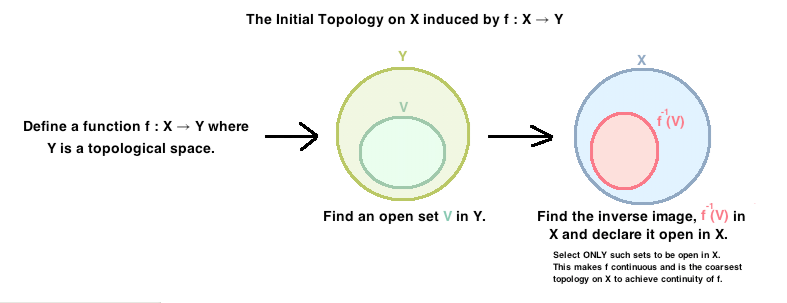
\includegraphics[scale = 0.5]{fotos_topo_1/topoinicial.png}
\end{equation}

Però necessitarem alguna cosa més a part d'una definició com la que hem donat per poder jugar amb aquestes topologies. El següent teorema ens donarà una subbase per a aquesta topologia. Cal destacar que a la classe de teoria de topologia es va donar aquest teorema com la definició de la topologia inicial.

\begin{ter}
\label{ter:topologiainicial} Sigui $X$ un conjunt i $\{(Y_i,\tau_i)\;:\;i\in I\}$ una col·lecció d'espais topològics, i $\{f_i\;:\;i\in I\}$ una col·lecció d'aplicacions. Aleshores la topologia inicial induïda per $\{f_i\;:\;i\in I\}$ en $X$ té la subbase
\begin{equation}
    \notag
    S = \{f_i^{-1}(U)\;:\;U\in\tau_i\}
\end{equation}
Alternativament, podem dir que té com a base
\begin{equation}
    \notag
    \beta_X = \{f_1^{-1}(U_1)\cap\cdots\cap f_n^{-1}(U_n)\;:\;U_i\;\text{obert de}\;Y_i,\;i=1,\ldots,n\} .
\end{equation}
\end{ter}
\begin{proof}
Per veure que la topologia inicial induïda per $\{f_i\;:\;i\in I\}$ en $X$ té la subbase $S$ hem de provar que la topologia $\tau$ generada per aquesta subbase és igual a la inicial induïda en $X$. Per fer això, hem de provar que $\tau$ és la topologia que fa cada aplicació $f_i:X\rightarrow Y_i$ continua, $\forall i\in I$, i que aquesta $\tau$ és la més grollera que ho fa.
\begin{itemize}
    \item Clarament, la topologia $\tau$ generada per la subbase $S$, o per la base $\beta$ (que està formada per interseccions finites d'elements de $S$) fa totes les $f_i:X\rightarrow Y_i$ perquè $\forall U\in \tau_i$ tenim $f_i^{-1}(U) \in \tau$ (és obert en $X$ respecte la topologia $\tau$ generada per $S$). Així, $\forall i\in I$, $f_i$ és contínua.
    \item Ara hem de veure que $\tau$ és la topologia més grollera que compleix això. Suposem que $\tau'$ és una altra topologia que fa que $f_i:X\rightarrow Y_i$ sigui continua per tot $i\in I$. Aleshores, $f_i^{-1}(U)\in \tau'$ per tot $i\in I$. Però com $\tau'$ és una topologia en $X$, compleix que totes les interseccions finites de $\tau'$ és de $\tau'$, per la definició (\ref{def:topologia}) de topologia, és a dir, que les interseccions finites dels $f_i^{-1}(U_i)$ estan en $\tau'$. Així, $\tau\subseteq\tau'$.
\end{itemize}
Per tant, qualsevol possible $\tau'$ que també compleix que fa contínues les $f_i$ per tot $i\in I$, ha de contenir $\tau$. Així que la topologia inicial $\tau$ induïda per $\{f_i\;:\;i\in I\}$ en $X$ té subbase $S = \{f_i^{-1}(U)\;:\;U\in\tau_i\}$.
\end{proof}

\begin{ej}
\label{ej:topoinicialinclusio} Si $X$ és un espai topològic i $Y\subseteq X$ és un subconjunt, la topologia subespai de $Y$ coincideix amb la topologia inicial respecte la inclusió
\begin{equation}
    \notag
    Y\overset{\iota}{\hookrightarrow} X
\end{equation}
En efecte, si $U\subseteq X$ és un obert, aleshores $Y\cap U = \iota^{-1}(U)$.
\end{ej}

\begin{prop}
\label{prop:composiciotopoinicial} Suposem que $Y$ està dotat de la topologia inicial respecte a $f_j:Y\rightarrow X_j$, $j = 1,\ldots,n$. Sigui $Z$ un espai topològic i $g:Z\rightarrow Y$ una aplicació. Aleshores, $g$ és contínua, si i només si, $f_1\circ g,\ldots, f_n\circ g$ són contínues.
\end{prop}
\begin{proof}
Doble implicació:
\begin{enumerate}[($\Rightarrow$)]
    \item És conseqüència del fet que la composició d'aplicacions contínues és contínua (\ref{prop:composiciodecontinues}).
\end{enumerate}
\begin{enumerate}[($\Leftarrow$)]
    \item Per veure que $g$ és contínua podem comprovar la continuïtat de $g$ utilitzant els oberts de la base donada a l'observació anterior. És suficient doncs veure que $\forall U\in \beta_Y$, $g^{-1}(U)$ és obert de $Z$. Ara bé,
    \begin{equation}
        \notag
        g^{-1}(f_{i_1}^{-1}(U_{i_1})\cap \cdots\cap f_{i_n}^{-1}(U_{i_n})) = (f_{i_1}\circ g)^{-1}(U_{i_1})\cap\circ\cap(f_{i_n}\circ g)^{-1}(U_{i_n}).
    \end{equation}
\end{enumerate}
\end{proof}



\subsection{Topologia final}
A l'apartat anterior hem vist que donat un conjunt $X$, un espai topològic $Y$ i una aplicació $f:X\rightarrow Y$, aleshores la topologia inicial induïda per $f$ a $X$ és la topologia més grollera que fa $f$ contínua. Més en general, si tenim un conjunt $X$, una col·lecció d'espais topològics $\{Y_i\}_{i\in I}$ i una col·lecció d'aplicacions $\{f_i\}_{i\in I}$ aleshores la topologia inicial induïda per les $f_i$ a $X$ és la més grollera que fa $f_i:X\rightarrow Y_i$ sigui contínua, $\forall i \in I$. També vam veure que la topologia inicial induïda per $\{f_i\}_{i\in I}$ a $X$ tenia com a subbase 
\begin{equation}
    \notag
    S = \{f_i^{-1}(U)\;:\;U\in\tau_i\}
\end{equation}
i, que per tant tenia com a base
\begin{equation}
    \notag
    \beta_X = \{f_1^{-1}(U_1)\cap\cdots\cap f_n^{-1}(U_n)\;:\;U_1,\ldots,U_n\;\text{oberts de}\;Y_1,\ldots,Y_n\;\text{resp.}\}
\end{equation}
A continuació, veurem una topologia bastant anàloga anomenada topologia final.

\begin{defi}[Topologia final]
\label{def:topologiafinal}\index{Topologia final} Sigui $X$ un conjunt i $\{Y_i\;:\;i\in I\}$ una família d'espais topològics i $\{f_i:Y_i\rightarrow X\;:\;i\in I\}$ una col·lecció d'aplicacions. La \textit{topologia final induïda per} $\{f_i\}_{i\in I}$ en $X$ és la topologia més fina $\tau$ en $X$ que fa que $f_i:Y_i\rightarrow X$ sigui contínua, $\forall i\in I$.
\end{defi}

És important emfatitzar que la topologia final induïda per $\{f_i\}_{i\in I}$ és la MÉS FINA que fa que $f_i:Y_i\rightarrow X$ sigui contínua $\forall i\in I$.

Per construir la topologia final a $X$ induïda per les aplicacions $f_i:Y_i\rightarrow X$, considerem qualsevol subconjunt $U$ de $X$. Prenem la antiimatge de $U$ respecte cadascuna de les $f_i$, és a dir, $f_i^{-1}(U)$. Si $f_i^{-1}(U)$ és obert en $Y_i$ en cada $i\in I$, aleshores declarem $U$ com a obert de $X$:

\begin{equation}
    \notag
    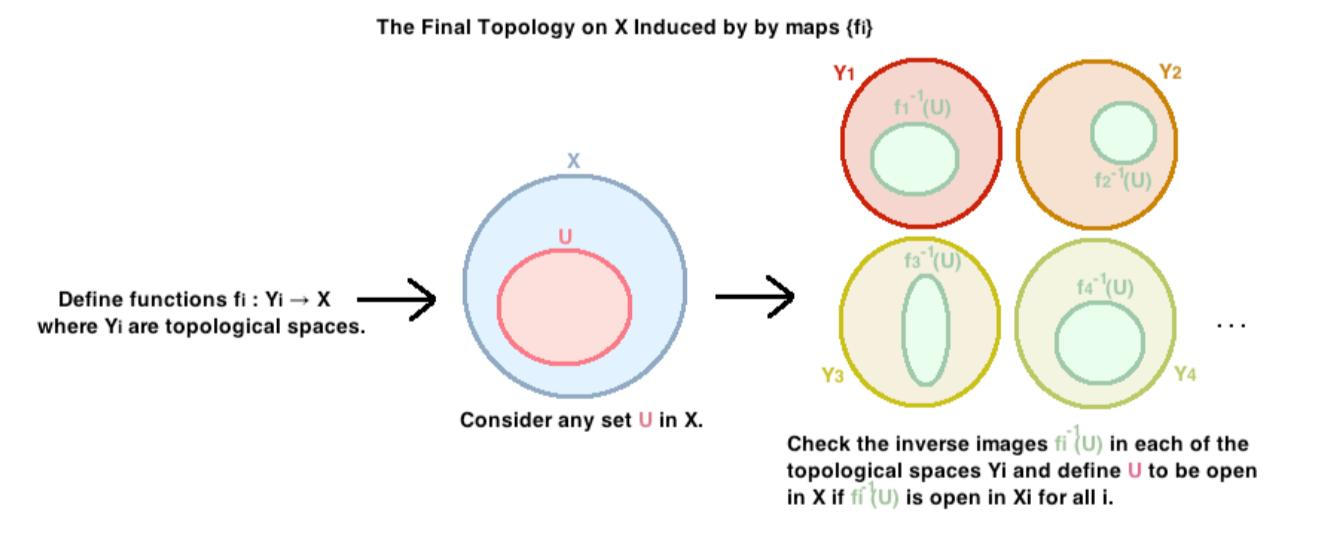
\includegraphics[scale=0.3]{fotos_topo_1/topofinal.jpeg}
\end{equation}

El següent teorema ens donarà una forma explícita per a la topologia final induïda per $\{f_i\}_{i\in I}$ en $X$.

\begin{ter}
\label{ter:topologiafinal} Sigui $X$ un conjunt, $\{(Y_i,\tau_i)\}_{i\in I}$ una col·lecció d'espais topològics i $\{f_i:Y_i\rightarrow X\}_{i\in I}$ una col·lecció d'aplicacions. Aleshores, la topologia final induïda per $\{f_i\}_i$ a $X$ ve donada per $\tau = \{U\subseteq X\;:\;f_i^{-1}(U)\in\tau_i,\;\forall i\in I\}$.
\end{ter}
\begin{proof}
Per provar que $\tau$ és la topologia final induïda per $\{f_i\}_{i\in I}$ en $X$ hem de veure que $\tau$ fa contínua $f_i:Y_i\rightarrow X$, per tot $i\in I$, i que qualsevol altra topologia $\tau'$ que també ho faci sigui més grollera que $\tau$.
\begin{itemize}
    \item Clarament, $f_i:Y_i\rightarrow X$ és contínua amb aquesta topologia ja que per tot $U\in \tau$ tenim que $f_i^{-1}(U)$ és obert $\forall i \in I$. Així que $f_i$ és contínua $\forall i\in I$.
    \item Ara suposem que $\tau'$ és una altra topologia que ho compleix. Si $\tau\varsubsetneq \tau'$, existeix $V\in\tau'$ tal que $v\not\in\tau$. Aleshores, si $V\in\tau'$, $V$ és obert de $X$, però ara $f_i^{-1}(V)$ no pot ser obert de $Y_i$ per tot $i\in I$, perquè sinó $V\in\tau$ per com està definida $\tau$. Això implica que $f_i$ no serà contínua, per algun $i$, i aleshores $\tau'$ no satisfà ser la topologia que fa totes les $f_i$ contínues. Per tant, $\tau\not\subseteq\tau'$ i així $\tau'\varsubsetneq \tau$.
\end{itemize}
Així que qualsevol topologia $\tau'$ en $X$ que també fa $f_i:Y_i\rightarrow X$ contínua per tot $i\in I$ ha de ser més grollera que $\tau$, per tant $\tau$ és la topologia final.
\end{proof}

\begin{prop}
\label{prop:topologiafinal} Amb les mateixes hipòtesis i la mateixa notació, sigui $g:X\rightarrow Z$ una aplicació entre espais topològics. Aleshores $g$ és contínua si i només si $g\circ f_i$ són contínues per a tot $i=1,\ldots,n$.
\end{prop}
\begin{proof}
Si $g$ és contínua, $g\circ f_i$ és composició d'aplicacions contínues. Recíprocament, sigui $U$ un obert de $Z$. Per definició de topologia final, $g^{-1}(U)$ és obert si, i només si, $f_i^{-1}(g^{-1}(U))$ és obert per a tot $i$, la qual cosa es verifica per la continuïtat de les aplicacions $g\circ f_i$.
\end{proof}



\subsection{Identificació}

\begin{defi}
[Identificació]\label{def:identificacio}\index{Identificació}Una \textit{identificació} és una aplicació contínua i exhaustiva $f:X\rightarrow Y$ tal que $Y$ té la topologia final respecte de $f$.
\end{defi}

\begin{prop}
\label{prop:identificacio} Sigui $f:X\rightarrow Y$ una aplicació contínua, exhaustiva i oberta (respectivament tancada). Aleshores $f$ és una identificació.
\end{prop}
\begin{proof}
Només cal veure que $Y$ té la topologia final, és a dir, que si $U\subset Y$ verifica que $f^{-1}(U)$ és un obert, aleshores $U$ és obert. Suposem que $f$ és oberta, per l'exhaustivitat $I=f(f^{-1}(U))$, i, per tant, $U$ és obert. Suposem ara que $f$ és tancada, novament per ser exhaustiva tenim que $f(X\setminus f^{-1}(U)) = Y\setminus U$. Així, $Y\setminus U$ és tancat i, per tant, $U$ és obert.
\end{proof}
\begin{ej}
\label{ej:topologiafinal} $X = [0,1]$, $Y = S^1$, $f(t) = (\cos(2\pi t),\sin(2\pi t))$. L'aplicació $f$ és contínua i exhaustiva, i tancada. Per la proposició és una identificació.
\end{ej}

Més endavant veurem exemples d'identificacions d'espais topològics en el conjunt de les seves classes per una relació d'equivalència definida a aquest espai.



\section{Topologia subespai}
Recordem de la topologia inicial que si $X$ és un conjunt, $\{Y_i\}_{i\in I}$ una col·lecció d'espais topològics i $\{f_i\}_{i\in I}$ una col·lecció d'aplicacions, aleshores la topologia inicial induïda per $\{f_i\}_{i\in I}$ en $X$ és la topologia $\tau$ més grollera que fa $f_i:X\rightarrow Y_i$ contínua per tot $i\in I$.

A continuació veurem un tipus molt important de topologia: La topologia subespai. Tot i que ja es va donar aquesta definició a (\ref{def:topologiasubespai}) la torno a escriure perquè ara, al context en el que estem, crec que s'entén millor, sabent tot el que sabem de la topologia inicial. També veurem més exemples i aplicacions que no s'han vist i que a classe no s'han donat.

\subsection{Definició alternativa de subespai topològic}

\begin{defi}
[Topologia subespai]\label{def:topologiasubespai2.0} Sigui $(X,\tau)$ un espai topològic i $A\subseteq X$. La \textit{topologia subespai} en $A$ és la topologia donada per $\tau_A = \{A\cap U\;:\;U\in\tau\}$.
\end{defi}

Però amb aquesta definició no queda del tot clar si $\tau_A$ és realment la topologia d'un espai topològic $(A,\tau_A)$. Al proper teorema veurem que la topologia subespai $\tau_A$ és, de fet, una topologia en $A$.

\begin{ter}
\label{ter:topologiasubespai2.0} Sigui $(X,\tau)$ un espai topològic i $A\subseteq X$. Aleshores, $\tau_A=\{U\cap A\;:\;U\in\tau\}$ és una topologia en $A$.
\end{ter}
\begin{proof}
Sigui $A$ un subconjunt de l'espai topològic $X$ i considerem la inclusió
\begin{equation}
    \notag
    \iota:A\rightarrow X
\end{equation}
definida per $\iota(a) = a,\;\forall a\in A$. La topologia inicial induïda en $A$ per $\iota$ és la topologia més grollera que fa que $\iota:A\rightarrow X$ sigui contínua. aquesta topologia té com a subbase 
\begin{equation}
    \notag
    S= \{\iota^{-1}(U)\;:\;U\in\tau\} ,
\end{equation}
pel que vam veure a (\ref{ter:topologiainicial}). Com $U$ és obert de $X$ i $A\subseteq X$, tenim que 
\begin{equation}
    \notag
    \iota^{-1}(U) = A\cap U\quad \forall U\in\tau. 
\end{equation}
Per tant, $\tau_A = \{A\cap U\;:\;U\in\tau\}$ és a dir, la topologia subespai $\tau_A$ és de fet la topologia inicial induïda per $\iota$.
\begin{equation}
    \notag
    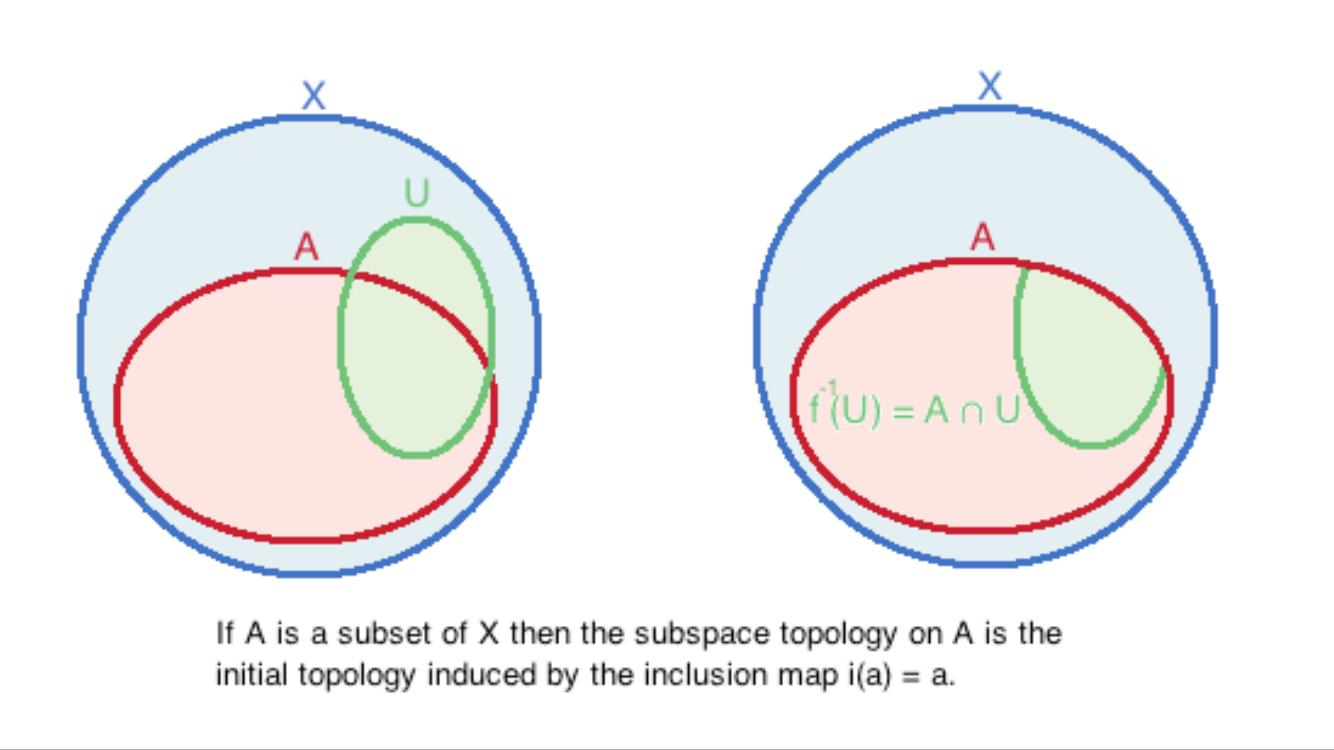
\includegraphics[scale = 0.3]{fotos_topo_1/topologiasubespai1.jpeg}
\end{equation}
\end{proof}

\begin{defi}
[Subespai topològic]\label{def:subespaitopologic}\index{Subespai topològic} Sigui $(X,\tau)$ un espai topològic i $A\subseteq X$ un subconjunt dotat de la topologia $\tau_A$ subespai. Aleshores, $(A,\tau_A)$ és un espai topològic que anomenarem \textit{subespai topològic} de $X$. Normalment direm que $A$ és subespai topològic de $X$, i haurem d'entendre que $A$ està dotat de la topologia subespai.
\end{defi}

\begin{prop}
[Transitivitat de subespais]\label{prop:transitivitatdesubespais} Sigui $(X,\tau)$ un espai topològic. Si $Y$ és un subespai topològic de $X$ i $Z$ és un subespai topològic de $Y$, aleshores $Z$ és un subespai topològic de $X$.
\end{prop}

\begin{ej}
\label{ej:topologiasubespai1} Considerem l'espai topològic $(\mathbb{R}^2,\tau_e)$, on $\tau_e$ és la topologia usual dels discs oberts de $\mathbb{R}^2$. Determinem quina és la topologia subespai per al subconjunt
\begin{equation}
    \notag
    A = \{(x,0)\in\mathbb{R}^2\;:\;x\in\mathbb{R}\}\subset\mathbb{R}^2
\end{equation}

Notem que $A$ és simplement la recta real $\mathbb{R}$. Geomètricament, podem veure que la topologia subespai $\tau_A$ serà simplement la topologia usual a $\mathbb{R}$. Per veure això, considerem qualsevol obert a $\mathbb{R}$ amb la topologia usual d'intervals oberts a $\mathbb{R}$. Aleshores, qualsevol interval obert $(a,b)\subset\mathbb{R}$ pot ser construit prenent un disc obert de $\mathbb{R}^2$ que intersequi amb la recta $y=0$ als punts $(a,0),(b,0)$:
\begin{equation}
    \notag
    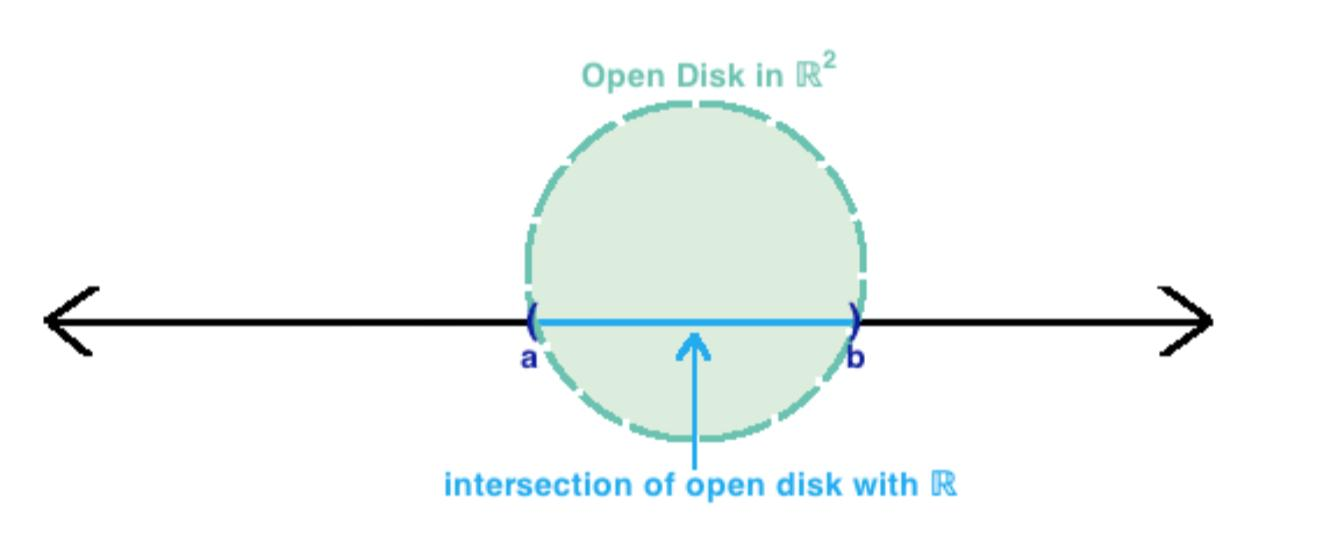
\includegraphics[scale = 0.3]{fotos_topo_1/topologiasubespai2.jpeg}
\end{equation}
Com que tot obert de $\mathbb{R}$ és una unió d'aquests intervals oberts, podem veure que la topologia subespai és simplement la topologia usual a $\mathbb{R}$.
\end{ej}

\begin{ej}
\label{ej:topologiasubespai2} Considerem l'espai topològic $(\mathbb{R},\tau)$, on $\tau$ és la topologia usual dels intervals oberts a $\mathbb{R}$. Hem de veure que la topologia subespai en $\mathbb{Z}\subset\mathbb{R}$ és la topologia discreta en $\mathbb{Z}$.

En efecte, sigui $x\in\mathbb{Z}$. Aleshores, l'interval obert $(x-1/2,x+1/2)\cap\mathbb{Z} = \{x\}$. Aleshores tot singletó $\{x\} $ està contingut a la topologia subespai en $\mathbb{Z}$. Però això implica que $\tau_\mathbb{Z}$ és la topologia discreta a $\mathbb{Z}$.
\end{ej}

\begin{ej}
\label{ej:topologiasubespai3} Sigui $X$ un conjunt dotat de la topologia discreta $\tau$ i sigui $A\subseteq X$ un subconjunt. El subespai topològic $(A,\tau_A)$ també té la topologia discreta (en $A$).

En efecte, sigui $A\subseteq X$. Per veure que $A$ té la topologia discreta en $A$, el que hem de veure és que tot subconjunt d'$A$ és obert en $A$. Sigui $U\subseteq A$ un obert de $A$. Aleshores $U\subseteq X$. Per tant, $U$ és obert de $X$. A més, $A\cap U = U$ és obert de $A$, per tant $\tau_A$ és la topologia discreta en $A$.
\end{ej}

\begin{ej}
\label{ej:topologiasubespai4} Sigui $(X,\tau)$ un espai topològic i $A\subseteq X$. Aleshores $\tau_A\subseteq \tau \Leftrightarrow A\in\tau$.

Suposem que $\tau_A\subseteq\tau $. Com $A$ és un obert en $A$, $A\in\tau_A\Rightarrow A\in\tau$.

Recíprocament, suposem que $A\in\tau$. Sigui $U\in\tau_A$. Aleshores $U$ és obert de $A$. Llavors existeix un obert $V\subset X$ tal que $U = A\cap V$. Però $A$ és obert en $X$ ja que $A\in\tau$, així que $A\cap V = U$ és obert en $X$ (la intersecció finita d'oberts és obert). Per tant, $U\in\tau$, ergo $\tau_A\subseteq \tau$.
\end{ej}

\subsection{Oberts i tancats en subespais topològics}

Recordem que si $(X,\tau)$ és un espai topològic i $A\subseteq X$, aleshores podem definir una topologia $\tau_A$ en $A$ anomenada la topologia subespai en $A$ explicitada com
\begin{equation}
    \notag
    \tau_A = \{A\cap U\;:\;U\in\tau\} .
\end{equation}
Junts, $(A,\tau_A)$ formen el que anomenem subespai topològic. Notem que, per la definició, un subconjunt $V\subseteq A$ és obert en $A$ amb la topologia subespai $\tau_A$ si, i només si, existeix un obert $U$ en $X$ tal que $V = A\cap U$. Aleshores, que se'n pot dir dels tancats d'$A$? El següent teorema ens dona exactament el que esperem.

\begin{ter}
\label{ter:subespaitopologic1} Sigui $(X,\tau)$ un espai topològic i sigui $A\subseteq X$. Un subconjunt $C\subseteq A$ és tancat en $A$ si i només si existeix un tancat $D$ de $X$ tal que $C = A\cap D$.
\end{ter}
\begin{proof}
\begin{enumerate}[($\Rightarrow$)]
    \item Sigui $C\subseteq A$ un tancat d'$A$. Aleshores $A\setminus C$ és obert en $A$. Per tant, existeix un obert $U$ en $X$ tal que $A\setminus C = A\cap U$. Agafant el complementari a ambdues bandes respecte $A$ tenim
    \begin{equation}
        \notag
        A\setminus(A\setminus C) = A\setminus(A\cap U)\Longrightarrow C = A\cap U^c
    \end{equation}
    Així que sigui $D = U^c$ i obtenim el que volíem: $D$ és tancat a $X$ i $C = A\cap D$.
\end{enumerate}
\begin{enumerate}[($\Leftarrow$)]
    \item Suposem que existeix $D$ tancat de $X$ tal que $C = A\cap D$. Aleshores
    \begin{equation}
        \notag
        A\setminus C = A\setminus(A\cap D)\Longrightarrow A\setminus C = A\cap D^c
    \end{equation}
    on $D^c$ és un obert en $X$, aleshores $A\cap D^c$ és un obert en $A$. En altres paraules, $A\setminus C$ és obert en $A$, així que $C$ és tancat en $A$.
\end{enumerate}
\end{proof}

\subsection{Propietats hereditàries de subespais topològics}

Recordem que si tenim un espai topològic $(X,\tau)$ i $A\subseteq X$ un subconjunt, aleshores la topologia subespai $\tau_A$ ve donada com la col·lecció de les interseccions de tots els oberts de $X$ amb $A$, és a dir,
\begin{equation}
    \notag
    \tau_A = \{U\cap A\;:\;U\in\tau\} .
\end{equation}
Hem provat que $\tau_A$ és realment una topologia i que és la topologia inicial induïda per l'aplicació inclusió 
\begin{equation}
    \notag
    \begin{array}{rl}
        \iota:A & \rightarrow X \\
        a & \mapsto \iota(a) = a
    \end{array}
\end{equation}
(la topologia més grollera que fa $\iota$ contínua). Ara mirarem de classificar propietats de $(X,\tau)$ que es ``transmeten'' o es ``passen'' a $(A,\tau_A)$.

\begin{defi}
[Propietat hereditària]\label{def:hereditaria}\index{Propietat hereditària} Sigui $(X,\tau)$ un espai topològic. Una propietat de $(X,\tau)$ es diu \textit{hereditària} si per tot $A\subseteq X$ es compleix que el subespai topològic $(A,\tau_A)$ també satisfà aquesta propietat. Una propietat de $X$ que no sigui hereditària es dirà \textit{no-hereditària}.
\end{defi}

\subsubsection{Herència del primer axioma de numerabilitat}
Provarem a continuació que el primer axioma de numerabilitat és hereditari.

\begin{ter}
\label{ter:1anhereditari} El primer axioma de numerabilitat és hereditari. És a dir, si $(X,\tau)$ és un espai topològic que satisfà el primer axioma de numerabilitat i $A\subseteq X$ és un subconjunt, aleshores el subespai topològic $(A,\tau_A)$ també satisfà el primer axioma de numerabilitat.
\end{ter}
\begin{proof}
Sigui $(X,\tau)$ un espai topològic que satisfà el 1r AN. Sigui $A\subseteq X$. Com $X$ satisfà el 1r AN tenim que $\forall a\in A\subset X$ ($\Rightarrow a\in X$) té una base d'entorns numerable. Sigui $\beta_a$. Per a cada $a\in A$ afirmem que la següent col·lecció és una base d'entorns numerable d'$a\in A$ en $A$:
\begin{equation}
    \notag
    \Tilde{\beta_a} = \{A\cap B\;:\;B\in\beta_a\}
\end{equation}
Clarament és un conjunt numerable ja que $\beta_a$ és un conjunt numerable. Recordem que una col·lecció de conjunts és una base d'entorns d'$a\in A$ si per tot obert d'$A$ existeix un obert $V$ en $X$ tal que $a\in U = A\cap V$. Com $V$ és obert en $X$ i $\beta_a$ és una base d'entorns d'$a$ en $X$ tenim que existeix un conjunt $B\in\beta_a$ tal que $a\in B\subseteq V$. Finalment veiem que 
\begin{equation}
    \notag
    a\in A\cap B\subseteq A\cap V = U.
\end{equation}
El conjunt $A\cap B$ és un obert en $A$ (amb la topologia subespai $\tau_A$), així que, tot obert $U$ en $A$ i per tot $a\in U$ existeix un element $A\cap B\in \beta_a$ tal que $a\in A\cap B\subseteq U$, així que $\Tilde{\beta_a}$ és una base d'entorns de $a$ en $A$.
\end{proof}

\subsubsection{Herència del segon axioma de numerabilitat}
Veurem ara que el segon axioma de numerabilitat també és hereditari.

\begin{ter}
\label{ter:2anhereditari} El segon axioma de numerabilitat és hereditari. És a dir, si $(X,\tau)$ és un espai topològic que satisfà el segon axioma de numerabilitat i $A\subseteq X$ és un subconjunt, aleshores el subespai topològic $(A,\tau_A)$ també satisfà el segon axioma de numerabilitat.
\end{ter}
\begin{proof}
Sigui $(X,\tau)$ un espai topològic que satisfà el 2n AN i $A\subseteq X$. Aleshores existeix una base numerable $\beta$ de $X$. Afirmo que la següent col·lecció és una base numerable de $A$:
\begin{equation}
    \notag
    \beta_A = \{A\cap B\;:\;B\in\beta\}
\end{equation}
Clarament $\beta_A$ és numerable ja que $\beta$ és numerable. Només queda veure que és una base de $\tau_A$ en $A$. Per veure això hem de provar que tot obert d'$A$ (respecte la topologia subespai $\tau_A$) és unió d'una subcol·lecció de conjunts de $\beta_A$. Sigui $U\subseteq A$ un obert de $A$. Com $U$ és obert en $A$ i $A\subseteq X$ tenim que existeix un obert $V$ en $X$ tal que $U = A\cap V$. Com $V$ és obert en $X$ i $\beta$ és base de $X$, tenim que existeix $\beta^*\subseteq \beta$ tal que
\begin{equation}
    \notag
    V = \bigcup_{B\in\beta^*}B \Longrightarrow U =  A\cap \left(\bigcup_{B\in\beta^*}B\right) = \bigcup_{B\in\beta^*}(A\cap B)
\end{equation}
Ara, $A\cap B\in\tau_A$ per cada $B\in\beta^*\subset\beta$. Per tant, tot obert $U$ de $A$ pot ser expressat com a unió d'elements de $\beta_A$ i aleshores $\beta_A$ és una base de $\tau_A$ en $A$, com volíem veure.
\end{proof}

\section{Topologia suma}
\subsection{Suma topològica d'espais topològics}
Estudiarem ara un espai topològic que podem crear a partir d'altres espais topològics.

\begin{defi}
[Suma topològica]\label{def:sumatopologica}\index{Suma topològica}\index{Espai topològic suma}\index{Topologia suma} Sigui $\{(X_i,\tau_i)\;:\;i\in I\}$ una col·lecció d'espais topològics disjunts. La \textit{suma topològica} (o espai topològic dotat de la topologia suma, o espai topològic suma), denotat
\begin{equation}
    \notag
    \bigoplus_{i\in I} X_i,
\end{equation}
és l'espai topològic amb el conjunt 
\begin{equation}
    \notag
    \bigcup_{i\in I}X_i
\end{equation}
i la topologia $\tau$ donada per la base
\begin{equation}
    \notag
    \beta = \{U\subseteq \bigcup_{i\in I}X_i\;:\;U\in\tau_i,\;\text{per algun}\;i\in I\}. 
\end{equation}
\end{defi}

\begin{equation}
    \notag
    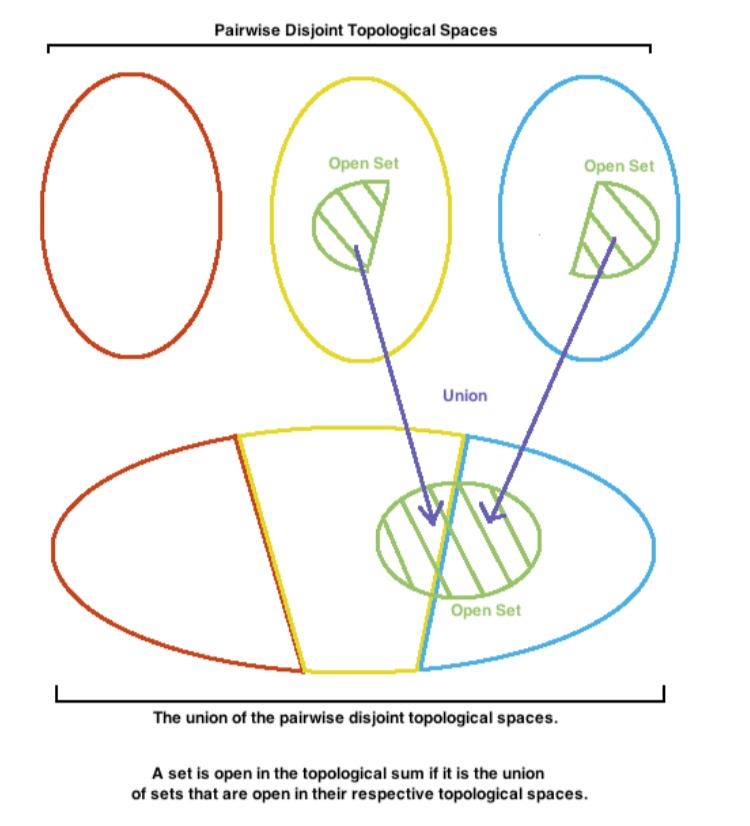
\includegraphics[scale = 0.3]{fotos_topo_1/topologiasuma.jpeg}
\end{equation}

\begin{ter}
\label{ter:topologiasuma} Sigui $\{(X_i,\tau_i)\;:\;i\in I\}$ una col·lecció d'espais topològics disjunts. Aleshores, un conjunt $V$ és obert a l'espai topològic suma $\bigoplus_{i\in I} X_i$ si, i només si, $U\cap X_i$ és obert de $\tau_i$, per a cada $i\in I$.
\end{ter}
\begin{proof}
Suposem que $V$ és obert en l'espai topològic suma $\bigoplus_{i\in I}$. Per la definició, tenim que la base de la topologia en $\bigoplus_{i\in I}X_i$ ve donada per 
\begin{equation}
    \notag
    \beta = \left\{U\subseteq\bigcup_{i\in I}X_i\;:\;U\in\tau_i,\;\text{per algun}\;i\in I\right\} .
\end{equation}
Aleshores, per algun $\beta^*\subseteq \beta$, tenim que
\begin{equation}
    \notag
    V = \bigcup_{B\in\beta^*}B.
\end{equation}
Cada $B\in\beta^*$ és tal que $B\in\tau_i$ per cert $i\in I$. Aleshores $V\cap X_i$ és o bé una unió arbitrària d'oberts de $X_i$, que és un obert en $X_i$, o bé és el buit (que també és obert). Per tant $V\cap X_i$ és obert per tot $i\in I$.

Recíprocament, suposem que $V\cap X_i$ és obert per tot $i\in I$. Aleshores, com els espais topològics $X_i$, $i\in I$ són disjunts, tenim
\begin{equation}
    \notag
    V = V\cap \bigcup_{i\in I}X_i = \bigcup_{i\in I}(V\cap X_i)
\end{equation}
Cadascun dels $V\cap X_i$ està a $\beta$, aleshores com $V$ és una unió arbitrària d'elements de la seva base (que són oberts) tenim que $V$ és obert en l'espai topològic suma $\bigoplus_{i\in I}X_i$.
\end{proof}



\section{Topologia producte}
\subsection{Topologia producte}
Siguin $(X,\tau_X)$ i $(Y,\tau_Y)$ dos espais topològics. Volem definir una topologia sobre el producte cartesià $X\times Y$. És natural demanar que, amb aquesta topologia, les projeccions
\begin{equation}
    \notag
    p_X:X\times Y\rightarrow X,\qquad p_Y:X\times Y\rightarrow Y
\end{equation}
siguin aplicacions contínues.

\begin{defi}
[Topologia producte]\label{defi:topologiaproducte}\index{Topologia producte} Siguin $(X,\tau_X)$ i $(Y,\tau_Y)$ dos espais topològics. La \textit{topologia producte} a $X\times Y$ és la topologia inicial a $X\times Y$ respecte a les projeccions $p_X:X\times Y\rightarrow X$ i $p_Y:X\times Y\rightarrow Y$.
\end{defi}

Per tant, la topologia producte a $X\times Y$ té per base
\begin{equation}
    \notag
    \beta_{X\times Y} = \{p_X^{-1}(U)\cap p_Y^{-1}(V) = U\times V\;:\;U\in\tau_X,\;V\in\tau_Y\} .
\end{equation}
Observem que aquesta $\beta_{X\times Y}$ en general no és una topologia, ja que poden existir elements $U,V\in\beta_{X\times Y}$ tals que $U\cup V\not\in\beta_{X\times Y}$. En canvi, la topologia inicial en un conjunt $Y$ respecte a una única aplicació $f:Y\rightarrow X$ té per conjunts d'oberts $\{f^{-1}(U)\;:\;U\in \tau_X\}$ (per exemple, quan definim la topologia subespai en un subconjunt d'un espai topològic).

\begin{ej}
Vegem-ne exemples:
\begin{enumerate}[(1)]
    \item Sigui $X = \mathbb{R}$ amb la topologia euclidiana. La topologia producte a $\mathbb{R}\times\mathbb{R}$ és la que té com a oberts reunions arbitràries de subconjunts de la forma $(a_1,b_1)\times(a_2,b_2)$ amb $a_1\leq b_1$ i $a_2\leq b_2$ (és a dir, producte cartesià d'intervals). Per tant, coincideix amb la topologia euclidiana d'$\mathbb{R}^2$. En particular, no tots els oberts són de la forma $U\times V$. 
    
    Anàlogament, la topologia producte sobre $\mathbb{R}\times\overset{n)}{\cdots}\times \mathbb{R}$ és la topologia euclidiana sobre $\mathbb{R}^n$.
    
    \item Si $(X,d_X)$ i $(Y,d_Y)$ són espais mètrics, la topologia associada a la mètrica producte
    \begin{equation}
        \notag
        d_{X\times Y}((a,b),(x,y)) :=\max\{d_X(a,x),d_Y(b,y)\}
    \end{equation}
    és la topologia producte.
\end{enumerate}
\end{ej}

Les dues projeccions anteriors impliquen:
\begin{prop}
\label{prop:topoproducte1} La topologia producte a $X\times Y$ és la més grollera respecte a la qual les dues projeccions $p_X, p_Y$ són contínues.
\end{prop}

\begin{prop}
\label{prop:topoproducte2} Si $X\times Y$ està dotat de la topologia producte i $Z$ és un espai topològic, aleshores una aplicació $g:Z\rightarrow X\times Y$ qualsevol si i només si les composicions $p_X\circ g$ i $p_Y\circ g$ són contínues.
\end{prop}

\begin{prop}
\label{prop:topoproducte3} Siguin $X,Y,Z$ espais topològics i $f:Z\rightarrow X$, $g:Z\rightarrow Y$ aplicacions. L'aplicació 
\begin{equation}
    \notag
    \begin{array}{rl}
        \varphi:Z & \rightarrow X\times Y \\
        z & \longmapsto (f(z),g(z))
    \end{array}
\end{equation}
és contínua si i només si $f$ i $g$ són contínues.
\end{prop}

Si $X$ i $Y$ són espais topològics, quan escrivim $X\times Y$ sobreentendrem (a menys que diguem el contrari) que parlem de la topologia producte.

Tot el que hem dit es generalitza de manera immediata al producte cartesià de $n$ espais topològics $X_1,\ldots,X_n$.

\begin{prop}
\label{prop:topoproducte4} Quan es tracta de dos espais topològics, es poden mirar dos productes: $X\times Y$ i $Y\times X$. Afortunadament, aquests dos espais topològics són homeomorfs. Un homeomorfisme explícit és $f:X\times Y\rightarrow Y\times X$ donat per $f(x,y) = (y,x)$.
\end{prop}
\begin{proof}
Per veure que $f$ és un homeomorfisme hem de veure que $f$ és contínua, bijectiva i que $f^{-1}$ és contínua.
\begin{itemize}
    \item No és molt difícil veure que és bijectiva: Sigui $(x,y),(z,w)\in X\times Y$ i suposem que $f(x,y) = f(z,w)$. Aleshores $(y,x) = (w,z)$ que implica que $y = w$ i $x = z$, és a dir $(x,y) = (z,w)$, per tant és injectiva.
    
    Sigui ara $(z,w)\in Y\times X$. Aleshores $f(w,z) = (z,w)$ que mostra que $f$ és exhaustiva i per tant és bijectiva.
    \item Veiem ara que $f$ és contínua. Sigui $V\times U\subseteq Y\times X$, on $V$ és obert en $Y$ i $U$ en $X$. Aleshores $f^{-1}(V\times U) = U\times V$. Però $U$ és obert en $X$ i $V$ és obert en $Y$, aleshores $U\times V$ és obert en $X\times Y$ i per tant ho és $f^{-1}(V\times U)$ i així $f$ és contínua.
    \item Sigui, per últim $U\times V\subseteq X\times Y$, on $U$ és obert de $X$ i $V$ és obert de $Y$. Aleshores $f(U\times V) = V\times U$ i com $V$ és obert en $Y$ i $U$ en $X$, aleshores $V\times U$ és obert en $Y\times X$ i per tant $f(U\times V) = (f^{-1})^{-1}(V\times U)$ és un obert en $X$ que implica que $f^{-1}$ és contínua.
\end{itemize}
\end{proof}

\begin{ej}
$\mathbb{R}^n\times\mathbb{R}^m\cong\mathbb{R}^{n+m}$. De fet, l'aplicació
\begin{equation}
    \notag
    \begin{array}{rl}
        \varphi:\mathbb{R}^n\times\mathbb{R}^m & \longrightarrow \mathbb{R}^{n+m} \\
        ((x_1,\ldots,x_n),(y_1,\ldots,y_m)) & \longmapsto (x_1,\ldots,x_n,y_1,\ldots,y_m)
    \end{array}
\end{equation}
és un homeomorfisme. En efecte:
\begin{enumerate}[(i)]
    \item $\varphi$ és una bijecció.
    \item Prenent com a base de la topologia euclidiana a $\mathbb{R}^{n+m}$ el conjunt
    \begin{equation}
        \notag
        \gamma = \{(a,b)\times\cdots\times(a_{n+m},b_{n+m})\;:\;a_i,b_i\in\mathbb{R}\},
    \end{equation}
    és clar que $\forall U\in\gamma$, $\varphi^{-1}(U)$ és un obert de $\mathbb{R}^n\times\mathbb{R}^m$ amb la topologia producte.
    
    \item $\varphi^{-1}$ és contínua perquè les composicions
    \begin{equation}
        \notag
        p_X\circ \varphi^{-1}:\mathbb{R}^{n+m}\rightarrow\mathbb{R}^n\times\mathbb{R}^m\rightarrow\mathbb{R}^n 
    \end{equation}
    \begin{equation}
        \notag
        p_Y\circ\varphi^{-1}:\mathbb{R}^{n+m}\rightarrow\mathbb{R}^n\times\mathbb{R}^m\rightarrow\mathbb{R}^m
    \end{equation}
    són contínues.
\end{enumerate}
\end{ej}

\begin{ej}\label{ej:tor}
El producte $S^1\times S^1$ s'anomena el \textit{tor}\index{Tor bidimensional}.
\begin{equation}
    \notag
    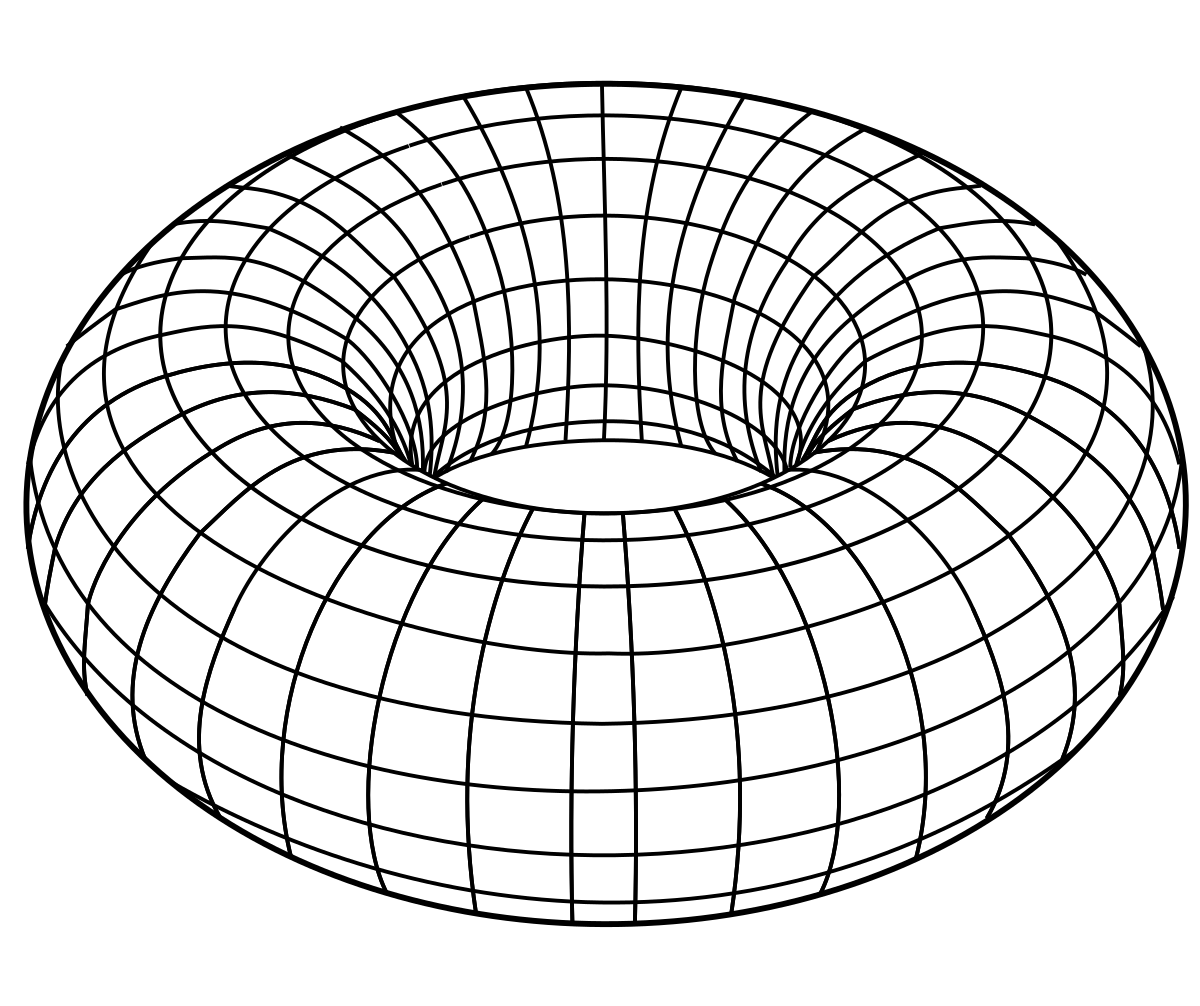
\includegraphics[scale = 0.1]{fotos_topo_1/tor.jpg}
\end{equation}
És homeomorf a $X = \{(x,y,z)\in\mathbb{R}^3\;:\;\left(\sqrt{x^2+y^2}-2\right)^2+z^2 = 1\}$.

En efecte, identificant $S^1 = \{(x,y)\in\mathbb{R}^2\;:\;x^2+y^2 = 1\}$, les aplicacions
\begin{equation}
    \notag
    \begin{array}{rl}
        f:S^1\times S^1 & \longrightarrow X \\
        ((a,b),(c,d)) & \longmapsto (a(c+2),b(c+2),d)
    \end{array}
\end{equation}
\begin{equation}
    \notag
    \begin{array}{rl}
        g:X & \longrightarrow S^1\times S^1 \\
        (x,y,z) & \longmapsto \left[\left(\frac{x}{\sqrt{x^2+y^2}},\frac{y}{\sqrt{x^2+y^2}}\right),\left(\sqrt{x^2+y^2}-2,z\right)\right]
    \end{array}
\end{equation}
són simultàniament inverses i, per tant, són bijeccions.
D'altra banda, $g$ és contínua perquè les composicions de $g$ amb les dues projeccions $S^1\times S^1\rightarrow S^1$ són contínues. Finalment, $f$ és contínua.
\end{ej}

\subsection{Oberts i tancats a la topologia producte}
Recordem que donada la col·lecció d'espais topològics $\{X_1,\ldots,X_n\}$ (finita) aleshores la topologia resultant del producte cartesià
\begin{equation}
    \notag
    \prod_{i=1}^n X_i = X_1\times \cdots\times X_n
\end{equation}
és la topologia donada per la base
\begin{equation}
    \notag
    \beta = \left\{\prod_{i=1}^n U_i\;:\;U_i\;\text{és obert de}\;X_i,\;i=1,\ldots,n\right\}. 
\end{equation}
Així doncs, els oberts de l'espai topològic producte són unions d'elements de $\beta$. Eles elements de la base són els oberts ``més simples'' de l'espai producte.

Però, quins són exactament els oberts de la base? Doncs, si $U_1,\ldots,U_n$ són oberts de $X_1,\ldots,X_n$ respectivament, aleshores $U_1\times \cdots\times U_n$ és un element de la base $\beta$.

\begin{ej}
\label{ej:topoproducteoberts} Considerem l'espai topològic $\mathbb{R}^n$. $\mathbb{R}^n$ és en realitat un espai producte:
\begin{equation}
    \notag
    \mathbb{R}^n = \mathbb{R}\times\overset{n)}{\cdots}\times \mathbb{R}
\end{equation}
i el següent conjunt és obert en $\mathbb{R}^n$ amb la topologia producte:
\begin{equation}
    \notag
    U = \prod_{i=1}^n (i,i+1) = (1,2)\times (2,3)\times\cdots\times (n,n+1)
\end{equation}
Fem $n=3$ per visualitzar-ho millor. Considerem 
\begin{equation}
    \notag
    U = (1,2)\times(2,3)\times (3,4)
\end{equation}
que és un obert en $\mathbb{R}^3$. Es pot representar de la següent manera:
\begin{equation}
    \notag
    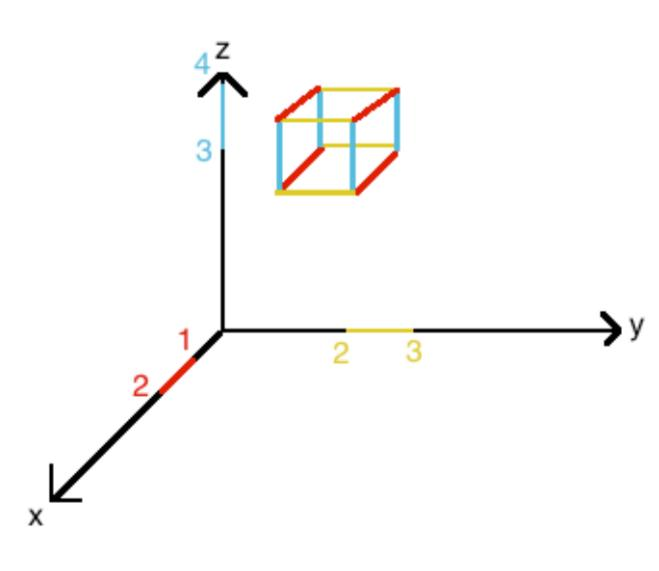
\includegraphics[scale = 0.3]{fotos_topo_1/topoprodoberts.jpeg}
\end{equation}
\end{ej}

Per tant, el producte d'oberts és un obert en l'espai producte. La següent proposició ens dirà un resultat anàleg pels tancats.

\begin{prop}
\label{prop:productetancats} Sigui $\{X_1,\ldots,X_n\}$ una col·lecció finita d'espais topològics. Si $C_i$ és un tancat de $X_i$, $i=1,\ldots,n$, aleshores el producte d'aquests tancats $C_1\times\cdots\times C_n$ és tancat a l'espai producte $X_1\times \cdots\times X_n$.
\end{prop}
\begin{proof}
Si $C_i$ és tancat a $X_i$ ($i=1,\ldots,n$) aleshores $X_i\setminus C_i$ és obert de $X_i$, per $i=1,\ldots,n$. Aleshores:
\begin{equation}
    \notag
    \left(\prod_{i=1}^nX_i\right)\setminus\left(\prod_{i=1}^n C\right) = 
\end{equation}
\begin{equation}
    \notag
    =\left[(X_1\setminus C_1)\times \cdots\times X_n\right]\cup\left[X_1\times(X_2\setminus C_2)\times \cdots\times X_n\right]\cup\cdots\cup\left[X_1\times\cdots\times (C_n\setminus X_n)\right]
\end{equation}
Això mostra que $\prod_i X_i \setminus \prod_i C_i$ és unió d'oberts en $X_1\times\cdots\times X_n$. Així doncs, és un obert en $X_1\times \cdots\times X_n$ i per tant $C_1\times \cdots\times C_n$ és un tancat.
\end{proof}

\subsection{L'interior, la clausura i la frontera de l'espai producte}

\subsubsection{Interior}
Al següent teorema veurem que donada una col·lecció finita $\{X_1,\ldots,X_n\}$ d'espais topològics i $A_i\subseteq X_i$, $\forall i\in \{1,\ldots,n\}$, aleshores l'interior del producte d'aquests conjunts és igual al producte de l'interior d'aquests conjunts.

\begin{ter}
\label{ter:interiorespaiproducte} Sigui $\{X_1,\ldots,X_n\}$ una col·lecció finita d'espais topològics i siguin $A_i\subseteq X_i$, $i\in\{1,\ldots,n\}$. Aleshores
\begin{equation}
    \notag
    \left(\prod_{i=1}^n A_i\right)^{o} = \prod_{i=1}^n A_i^{o}.
\end{equation}
\end{ter}
\begin{proof}
Sigui $x = (x_1,\ldots,x_n)\in A_1^{o}\times\cdots\times A_n^{o}$. Aleshores existeix un obert $U = U_1\times \cdots\times U_n$ en $X_1\times \cdots\times X_n$ tal que
\begin{equation}
    \notag
    x\in U = \prod_{i=1}^n U_i\subseteq\prod_{i=1}^n A_i .
\end{equation}
Aleshores, per tot $i\in\{1,\ldots,n\}$ tenim que $x_i\in U_i\subseteq X_i$. Cadascun dels oberts $U_i$ és obert en $X_i$, per tant $x_i\in X_i^{o},\;\forall i\in\{1,\ldots,n\}$. Així doncs $x\in\prod_{i=1}^n A_i^{o}$ que demostra que 
\begin{equation}
    \notag
    \left(\prod_{i=1}^n A_i\right)^{o}\subseteq\prod_{i=1}^n A_i^{o}
\end{equation}
Sigui ara $x = (x_1,\ldots,x_n)\in \prod_{i=1}^n A_i^{o}$. Aleshores $x_i\in A_i^{o}$ per cada $i\in\{1,\ldots,n\}$. Per tant, $\forall i$, existeix $U_i$ obert de $X_i$ tal que $x_i\in U_i\subseteq X_i$. Sigui
\begin{equation}
    \notag
    U = \prod_{i=1}^n U_i.
\end{equation}
Aleshores $U$ és obert en $\prod_{i=1}^n X_i$, ja que és producte d'oberts. A més, 
\begin{equation}
    \notag
    x\in U = \prod_{i=1}^n U_i\subseteq \prod_{i=1}^n A_i,
\end{equation}
per tant
\begin{equation}
    \notag
    x\in\left(\prod_{i=1}^n\right)^{o}
\end{equation}
que demostra que $\prod_{i=1}^n A_i^{o}\subseteq\left(\prod_{i=1}^n A_i\right)^{o}$ i per tant ja tenim la igualtat.
\end{proof}

\subsubsection{Clausura}
A continuació veurem que la clausura del producte és el producte de les clausures.

\begin{ter}
\label{ter:clausuraespaiproducte} Sigui $\{X_1,\ldots,X_n\}$ una família d'espais topològics i sigui $A_i\subseteq X_i,\;\forall i\in\{1,\ldots,n\}$. Aleshores 
\begin{equation}
    \notag
    \overline{\left(\prod_{i=1}^n A_i\right)} = \prod_{i=1}^n \overline{A_i}.
\end{equation}
\end{ter}
\begin{proof}
Suposem que $x = (x_1,\ldots,x_n)\in\overline{\left(\prod_{i=1}^n A_i\right)}$, $\forall i=1,\ldots, n$. Sigui $U_i$ un entorn obert de $x_i$. Aleshores, $U = \prod_{i=1}^n U_i$ és un entorn obert de $x$ i tenim que
\begin{equation}
    \notag
    \left(\prod_{i=1}^n A_i\right)\cap U = \left(\prod_{i=1}^n A_i\right)\cap\left(\prod_{i=1}^n U_i\right) = \prod_{i=1}^n(A_i\cap U_i)\not=\emptyset .
\end{equation}
Això implica que $A_i\cap U_i\not=\emptyset$, $\forall i=1,\ldots,n$. Per tant, $x_i\in \overline{A_i}$, $\forall i\in\{1,\ldots,n\}$, aleshores $x\in \prod_{i=1}^n \overline{A_i}$. Així,
\begin{equation}
    \notag
    \overline{\left(\prod_{i=1}^n A_i\right)}\subseteq \prod_{i=1}^n\overline{A_i}.
\end{equation}
Recíprocament, suposem ara que $x = (x_1,\ldots,x_n)\in \prod_{i=1}^n \overline{A_i}$. Per tant $x_i\in\overline{A}_i$ per tot $i\in\{1,\ldots,n\}$. Sigui $U = \prod_{i=1}^n U_i$ un entorn obert de $x$ en $X_1\times\cdots\times X_n$. Aleshores $U_i$ és un entorn obert de $x_i$, $\forall i = 1,\ldots, n$. Per tant, $A_i\cap U_i\not=\emptyset$ $\forall i$. Així doncs, obtenim que
\begin{equation}
    \notag
    \prod_{i=1}^n(A_i\cap U_i) = \left(\prod_{i=1}^n A_i\right)\cap\left(\prod_{i=1}^n U_i\right) = \left(\prod_{i=1}^n A_i\right)\cap U\not=\emptyset.
\end{equation}
Això demostra que $x\in\overline{\left(\prod_{i=1}^n A_i\right)}$ i per tant obtenim la inclusió contrària. Per tant obtenim la igualtat que buscàvem.
\end{proof}

\subsubsection{Conjunt de punts d'acumulació}
A continuació veurem que el producte dels conjunts de punts d'acumulació d'un conjunt està contingut al conjunt de punts d'acumulació del producte dels conjunts. Observem que en aquest cas només tenim una inclusió.

\begin{ter}
\label{ter:conjuntpuntsacumulacioespaiproducte} Sigui $\{X_1,\ldots,X_n\}$ una col·lecció finita d'espais topològics i $A_i\subseteq X_i,\;i\in\{1,\ldots,n\}$. Aleshores, 
\begin{equation}
    \notag
    \left(\prod_{i=1}^n A_i\right)'\supseteq \prod_{i=1}^n A_i'.
\end{equation}
\end{ter}
\begin{proof}
Sigui $x = (x_1,\ldots,x_n)\in\prod_{i=1}^n A_i'$. Aleshores $x_i\in A_i'$, per tot $i\in\{1,\ldots,n\}$. Sigui 
\begin{equation}
    \notag
    U = \bigcup_{i=1}^n U_i
\end{equation}
un entorn de $x$ en $\prod_{i=1}^n X_i$. Aleshores, cada $U_i$ és un entorn de cada $x_i$ respectivament. Per tant, 
\begin{equation}
    \notag
    (A_i\cap U_i)\setminus\{x_i\}\not=\emptyset \Longrightarrow \prod_{i=1}^n\left((A_i\cap U_i)\setminus\{x_i\}\right)\not=\emptyset.
\end{equation}
Per tant, 
\begin{equation}
    \notag
    \left(\prod_{i=1}^n A_i\right)\cap \left(\prod_{i=1}^n U_i\right)\setminus\{x\}\not=\emptyset.
\end{equation}
Així doncs, $x$ és un punt d'acumulació de $\prod_{i=1}^n A_i$, és a dir, $x\in\left(\prod_{i=1}^n A_i\right)'$ i per tant $\left(\prod_{i=1}^n A_i\right)'\supseteq\prod_{i=1}^n A_i'$.
\end{proof}


\section{Topologia quocient}
Recordem de (\ref{def:topologiafinal}) que si $X$ és un conjunt i $\{Y_i\}_{i\in I}$ una col·lecció arbitrària d'espais topològics, aleshores la topologia final induïda per $\{f_i:Y_i\rightarrow X\}_{i\in I}$ és la topologia $\tau$ més fina que fa les aplicacions
\begin{equation}
    \notag
    f_i:Y_i\rightarrow X
\end{equation}
contínues per tot $i\in I$. Recordem que vam veure que si $\tau$ era la topologia final induïda per $\{f_i\}_{i\in I}$, aleshores podia ser donada com
\begin{equation}
    \notag
    \tau = \{U\subseteq X\;:\;f^{-1}(U)\in\tau_i,\;\forall i\in I\} .
\end{equation}
Això és, la topologia final induïda per $\{f_i\}_{i\in I}$ és igual a la col·lecció de subespais de $X$ l'antiimatge dels quals està continguda en cada $\tau_i$, per $i\in I$.

\subsection{Topologia quocient}

Ara mirarem de definir un tipus especial de topologia en un conjunt coneguda com la topologia quocient. Abans, però, necessitem descriure una aplicació especial coneguda com aplicació quocient o pas al quocient o, simplement, quocient.

\begin{defi}
[Pas al quocient]\label{def:pasalquocient}\index{Pas al quocient} Sigui $(X,\tau)$ un espai topològic i sigui $\sim$ una relació d'equivalència a $X$. Per a cada $x\in X$, denotem la seva classe d'equivalència com $[x] = \{y\in X\;:\;x\sim y\}$ i sigui $X/\sim$ el conjunt de totes les classes d'equivalència. L'\textit{aplicació quocient} o \textit{pas al quocient} respecte el conjunt $X$ i la relació $\sim$ es defineix com l'aplicació
\begin{equation}
    \notag
    \begin{array}{rl}
        q:X & \longrightarrow X/\sim \\
        x & \longmapsto [x]
    \end{array}
\end{equation}
que envia cada element a la seva classe.
\end{defi}

\begin{equation}
    \notag
    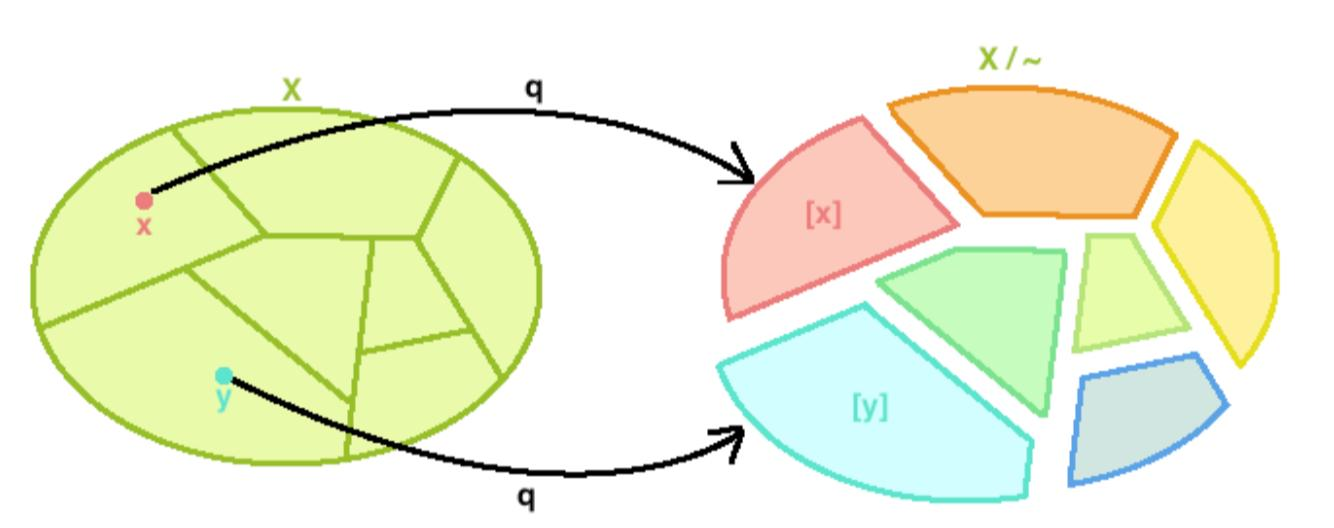
\includegraphics[scale = 0.3]{fotos_topo_1/topoquocient.jpeg}
\end{equation}

Ara ja estem preparats per definir la topologia quocient al conjunt de les classes d'equivalència $X/\sim$, on $\sim$ és una relació d'equivalència a $X$.

\begin{defi}
[Topologia quocient]\label{def:topologiaquocient}\index{Topologia quocient} Sigui $(X,\tau)$ un espai topològic i $\sim$ una relació d'equivalència a $X$. La \textit{topologia quocient} en $X/\sim$ és la topologia final induïda per l'aplicació quocient $q:X\rightarrow X/\sim$. Així, el resultant espai topològic $(X/\sim,\tau_\sim)$, anomenat \textit{espai topològic quocient}\index{Espai quocient}\index{Espai topològic quocient} és un espai topològic que té com a conjunt $X/\sim$ i com a topologia $\tau_\sim$ la topologia quocient.
\end{defi}

Veiem doncs que, la topologia quocient $\tau_\sim$ a $X/\sim$ és la topologia més fina que fa que l'aplicació pas al quocient $q:X\rightarrow X/\sim$ sigui contínua. Així doncs, ens trobem davant d'un cas particular de la topologia final (\ref{def:topologiafinal}). Als apunts del Naranjo això era un exemple o una observació a l'apartat d'identificacions i topologies finals.

\subsection{Oberts i tancats a la topologia quocient}
Els següents teoremes ens caracteritzaran quan un conjunt $U\subseteq X/\sim$ és obert o tancat.

\begin{ter}
\label{ter:topologiaquocientobert} Sigui $(X,\tau)$ un espai topològic i $\sim$ una relació d'equivalència a $X$. Sigui $X/\sim$ l'espai topològic quocient (dotat de la topologia quocient) respecte $\sim$. Aleshores $U\subseteq X/\sim$ és obert a $X/\sim$ si, i només si, 
\begin{equation}
    \notag
    \bigcup_{[x]\in U}[x]
\end{equation}
és obert en $X$.
\end{ter}
\begin{proof}
Per definició, la topologia quocient, sigui $\tau_q$, en $X/\sim$ és la topologia final al quocient $q:X\rightarrow X/\sim$ i es pot descriure com el següent conjunt:
\begin{equation}
    \notag
    \tau_q = \{U\subseteq X/\sim\;:\;q^{-1}(U)\in\tau\} .
\end{equation}

Aleshores, suposem que $U\subseteq X/\sim$ és obert en $X/\sim$. Per l'observació, $q^{-1}(U)$ és obert de $X$. I aleshores
\begin{equation}
    \notag
    q^{-1}(U) = \bigcup_{[x]\in U}[x].
\end{equation}
Per tant, $\bigcup_{[x]\in U}[x]$ és obert en $X$.

Recíprocament, sigui $U\subseteq X/\sim$ i suposem que $\bigcup_{[x]\in U}[x]$ és obert en $X$. Aleshores
\begin{equation}
    \notag
    q\left(\bigcup_{[x]\in U}[x]\right) = U.
\end{equation}
Aleshores $q^{-1}(U)$ és obert i com $q$ és oberta per la definició de $\tau_q$, tenim que $U$ és obert en $X/\sim$.
\end{proof}

\begin{ter}
\label{ter:topologiaquocienttancat}Amb les mateixes hipòtesis del teorema anterior, un conjunt $C\subseteq X$ és tancat en $X/\sim$ si, i només si $\bigcup_{[x]\in C}[x]$ és tancat en $X$.
\end{ter}
\begin{proof}
Bastant anàloga a la anterior, agafant complementaris de tancats que són oberts.
\end{proof}

\subsection{Topologia quocient en espais euclidians}

Ara veurem alguns exemples d'espais topològics quocients en espais euclidians, amb la topologia usual respectiva.

\begin{ej}
\label{ej:topologiaquocient1} Considerem $X = [0,1]$. Sigui $\tau_X$ la topologia usual d'intervals oberts en $X$ i considerem l'espai topològic $(X,\tau_X)$. Definim a $X$ la relació següent:
\begin{equation}
    \notag
    x\sim y \Leftrightarrow \left\{
    \begin{array}{cc}
        x = y \\
        \text{o bé}\\
        \{x,y\}=\{0,1\}
    \end{array}
    \right.
\end{equation}
Aquesta relació d'equivalència es pot pensar com ``enganxar'' els punts extrems de l'interval $[0,1]$ per formar com un cercle. És a dir, enganxem els punts que siguin equivalents (que són tots els punts amb ells mateixos i el zero amb l'1):
\begin{equation}
    \notag
    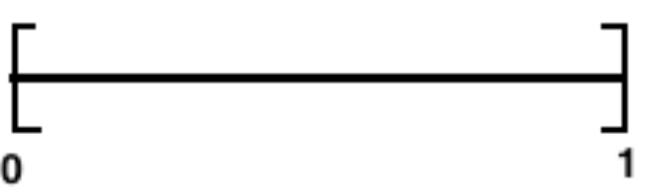
\includegraphics[scale = 0.2]{topoquocientexemple11.jpeg} \longrightarrow 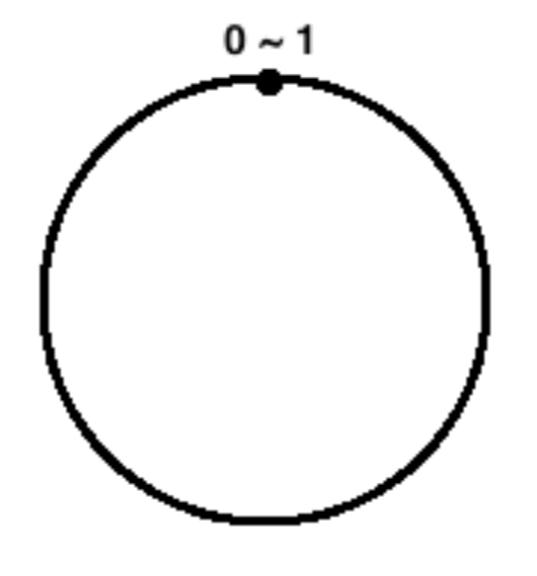
\includegraphics[scale = 0.2]{fotos_topo_1/topoquocientexemple12.jpeg}
\end{equation}
Notem que $\sim$ és efectivament una relació d'equivalència. És reflexiva, simètrica i transitiva clarament. Considerem doncs el conjunt de les classes d'equivalència
\begin{equation}
    \notag
    X/\sim = \{[x]\;:\;x\in[0,1]\}\cup\{\{0,1\}\} .
\end{equation}
Considerem l'aplicació pas al quocient $q:X\rightarrow X/\sim$ definida per tot $x\in [0,1]$ per $q(x) = [x]$. Aleshores, la topologia final induïda per $q$ és 
\begin{equation}
    \notag
    \tau_q = \{q^{-1}(U)\;:\;U\in \tau_X\} .
\end{equation}
Així doncs, la topologia $\tau_q$ pot ser descrita de forma informal com les unions ``d'arcs oberts'' que no contenen ni el 0 ni el 1, com indica el dibuix:
\begin{equation}
    \notag
    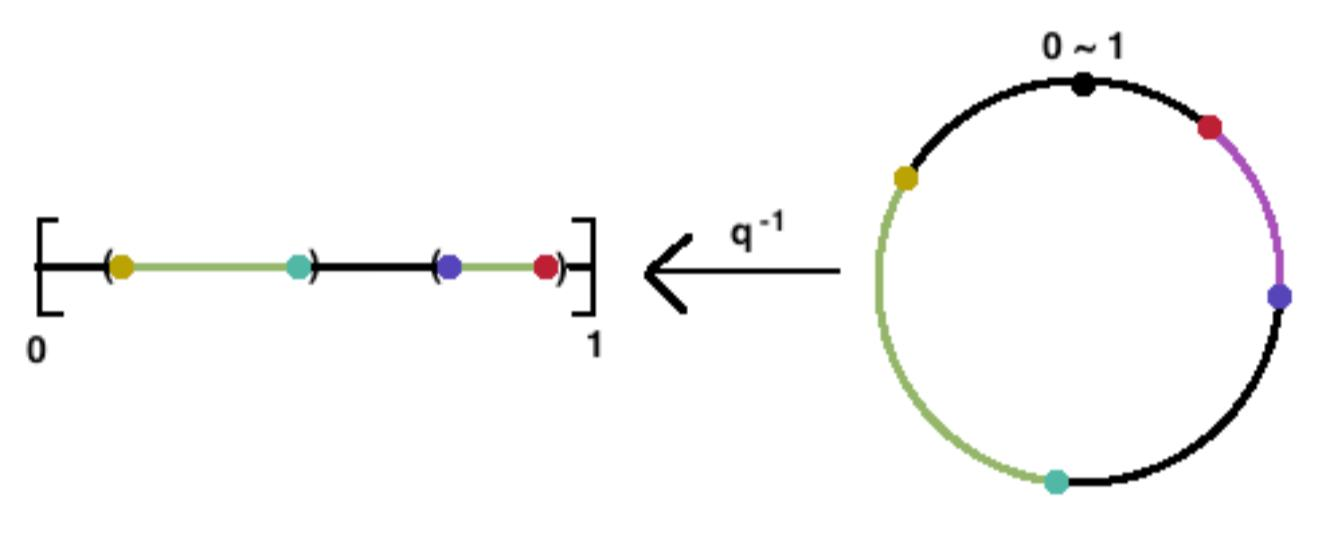
\includegraphics[scale = 0.3]{fotos_topo_1/topoquocientexemple13.jpeg}
\end{equation}
\end{ej}

\begin{ej}\label{ej:topologiaquocient2}
Considerem $X = [0,1]\times[0,1]$ i $(X,\tau_X)$ 
\begin{equation}
    \notag
    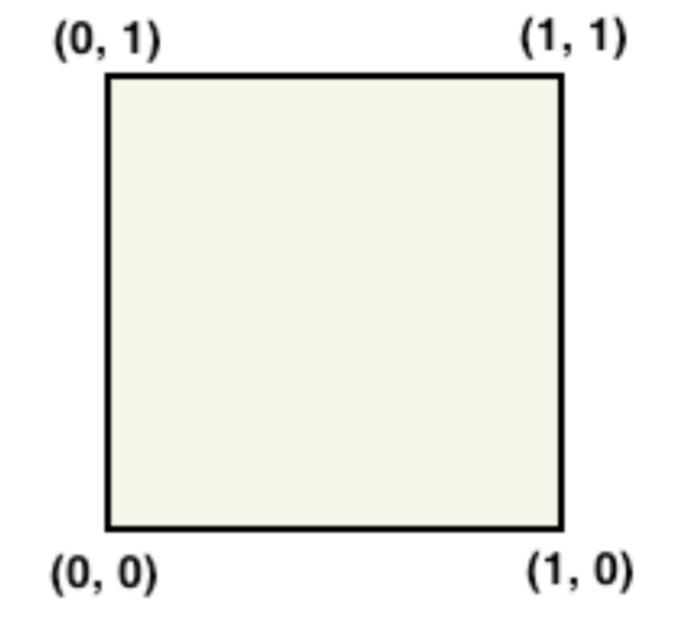
\includegraphics[scale = 0.3]{fotos_topo_1/topoquocientexemple21.jpeg}
\end{equation}
l'espai topològic on $\tau_X$ és la topologia usual dels discs oberts en $\mathbb{R}^2$. Definim la següent relació d'equivalència en $X$:
\begin{equation}
    \notag
    (x,y)\sim(w,z)\Leftrightarrow \left\{
    \begin{array}{rcl}
        x = w & \text{i} & \{y,z\} = \{0,1\} \\
        & \text{o bé} & \\
        y=z & \text{i} & \{x,w\} = \{0,1\}
    \end{array}
    \right.
\end{equation}
\begin{equation}
    \notag
    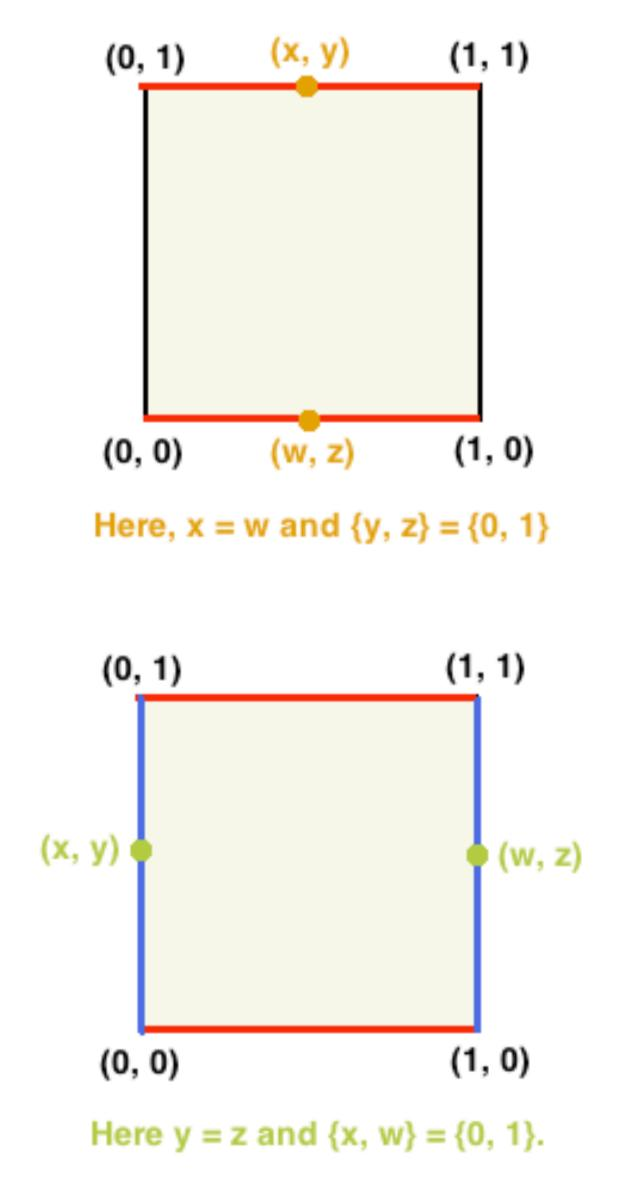
\includegraphics[scale = 0.3]{fotos_topo_1/topoquocientexemple22.jpeg}
\end{equation}
``Enganxant'' els punts equivalents junts podem visualitzar $X/\sim$ amb el següent diagrama:
\begin{equation}
    \notag
    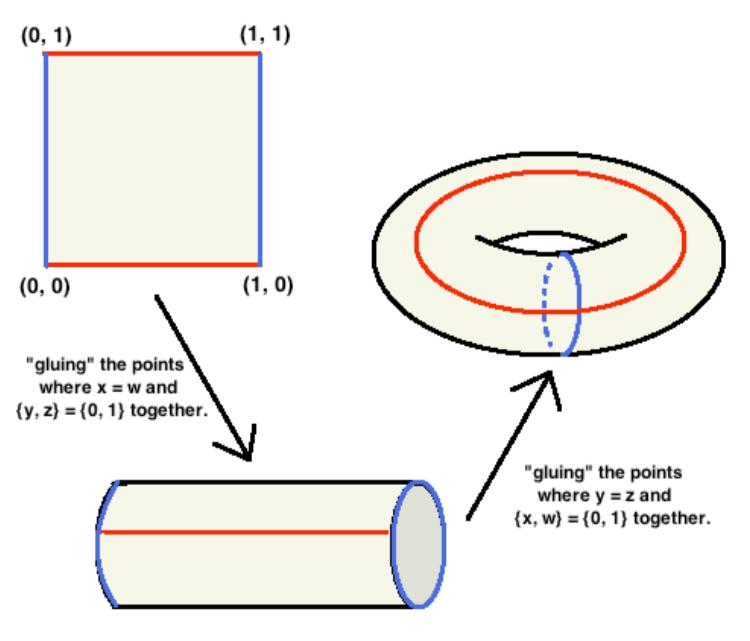
\includegraphics[scale = 0.3]{fotos_topo_1/topoquocientexemple23.jpeg}
\end{equation}
La topologia en $X/\sim$ serà generada per ``superfícies obertes'' del tor del dibuix, que no intersequin les ``línies d'enganxament''.
\end{ej}

\section{Espais localment euclidians}
\subsection{Espais localment euclidians}

Entre espais topològics destaquen pel seu interès geomètric els que localment tenen el mateix comportament que $\mathbb{R}^n$.

\begin{defi}
[Espais localment euclidians]\label{def:espaislocalmenteuclidians}\index{Espais localment euclidians} Un espai topològic és \textit{localment euclidià de dimensió $n$} si tot punt té un entorn obert homeomorf a la bola de $\mathbb{R}^n$ de centre 0 i radi 1.
\end{defi}

Observem que ser localment euclidià és una propietat invariant per homeomorfisme. Veurem exemples a les pròximes seccions.

\subsection{El lema de l'enganxament}

\begin{lema}
[Lema de l'enganxament]\label{lema:enganxament} Siguin $X$ i $Y$ i sigui $A,B\subseteq X$ subconjunts tancats de $X$ tals que $X = A\cup B$. Sigui $f:A\rightarrow Y$ i $g:B\rightarrow Y$ aplicacions contínues tals que $f(x) = g(x),\;\forall x\in A\cap B$. Aleshores la funció
\begin{equation}
    \notag
    h(x) = \left\{
    \begin{array}{rcl}
        f(x) & \text{si} & x\in A \\
        g(x) & \text{si} & x\in B
    \end{array}
    \right.
\end{equation}
és una funció contínua.
\end{lema}
Notem que és necessari que $f(x) = g(x),\;\forall x\in A\cap B$ per a que estigui ben definida.
\begin{equation}
    \notag
    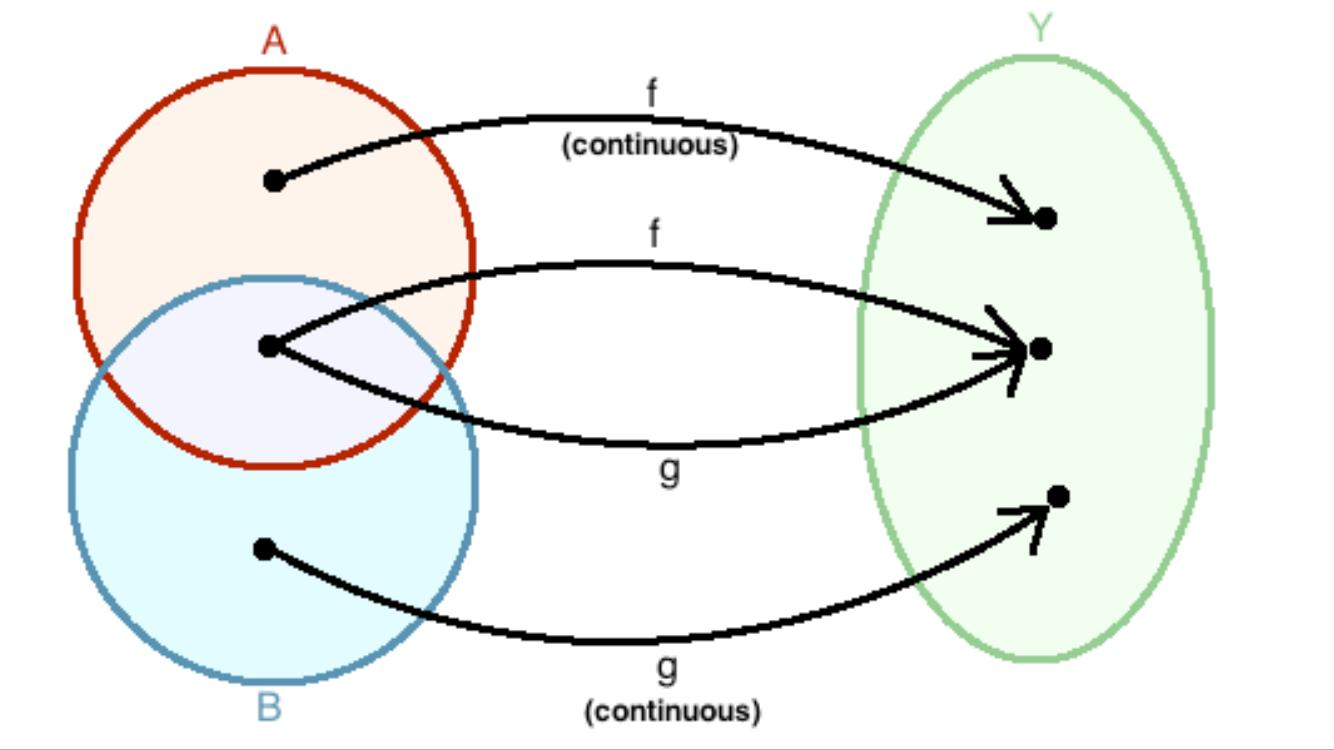
\includegraphics[scale = 0.3]{fotos_topo_1/gluinglemma1.jpeg}
\end{equation}
\begin{proof}
Per veure que $h$ és contínua, veurem que per tot tancat $V\subseteq Y$ tenim $h^{-1}(V)$ és tancat en $X$.

Sigui $V\subseteq Y$ un tancat. Aleshores
\begin{itemize}
    \item $f^{-1}(V)$ és tancat en $A$ perquè $f$ és contínua. Però com $A$ té la topologia subespai en $X$, existeix un tancat $F\subseteq X$ tal que $f^{-1}(V) = A\cap F$. Tenim que $A$ és tancat i per tant la intersecció aquesta és tancada en $X$.
    \item De manera similar, com $g$ és contínua, $g^{-1}(V)$ és tancat en $B$ que, de nou, té la topologia subespai en $X$ i per tant existeix un tancat $G\subseteq X$ tal que $g^{-1}(V) = G\cap B$ i la intersecció de tancats és tancada, així doncs, $g^{-1}(V)$ és un tancat en $X$.
\end{itemize}
Observem que, per a qualsevol $V\subseteq Y$ es compleix que $h^{-1}(V) = f^{-1}(V)\cup g^{-1}(V)$ i si prenem $V$ tancat, ambdós són tancats i per tant, la unió finita de tancats és tancat, això implica que $h^{-1}(V)$ és tancat en $X$.
\end{proof}

\subsection{Enganxant espais topològics a ells mateixos}

\begin{defi}
[Espai enganxament]\label{def:espaienganxament}\index{Espai enganxament} Sigui $Z$ un espai topològic i siguin $X$ i $Y$ subespais topològics disjunts de $Z$. Sigui $f:X\rightarrow Y$ una aplicació exhaustiva tal que $f(X) = Y$ és la imatge. Es defineix una relació d'equivalència $\sim$ per $x\sim y\Leftrightarrow f(x) = f(y)$ i $x\sim x,\;\forall x\in Z$. Aleshores les classes d'equivalència de $\sim$ són
\begin{equation}
    \notag
    \{\{y\}\cup f^{-1}(y)\;:\;y\in Y\},\qquad \text{i singletons} \quad \{y\} .
\end{equation}
L'espai resultant denotat $\mathcal{Z}_f$ es diu \textit{espai enganxament de $X$ i $Y$ a partir de $f$}.
\end{defi}

Molt sovint (als apunts del Naranjo-Navarro, per exemple) s'utilitza la notació $R_f$ per a la definició de $\sim$.

\begin{equation}
    \notag
    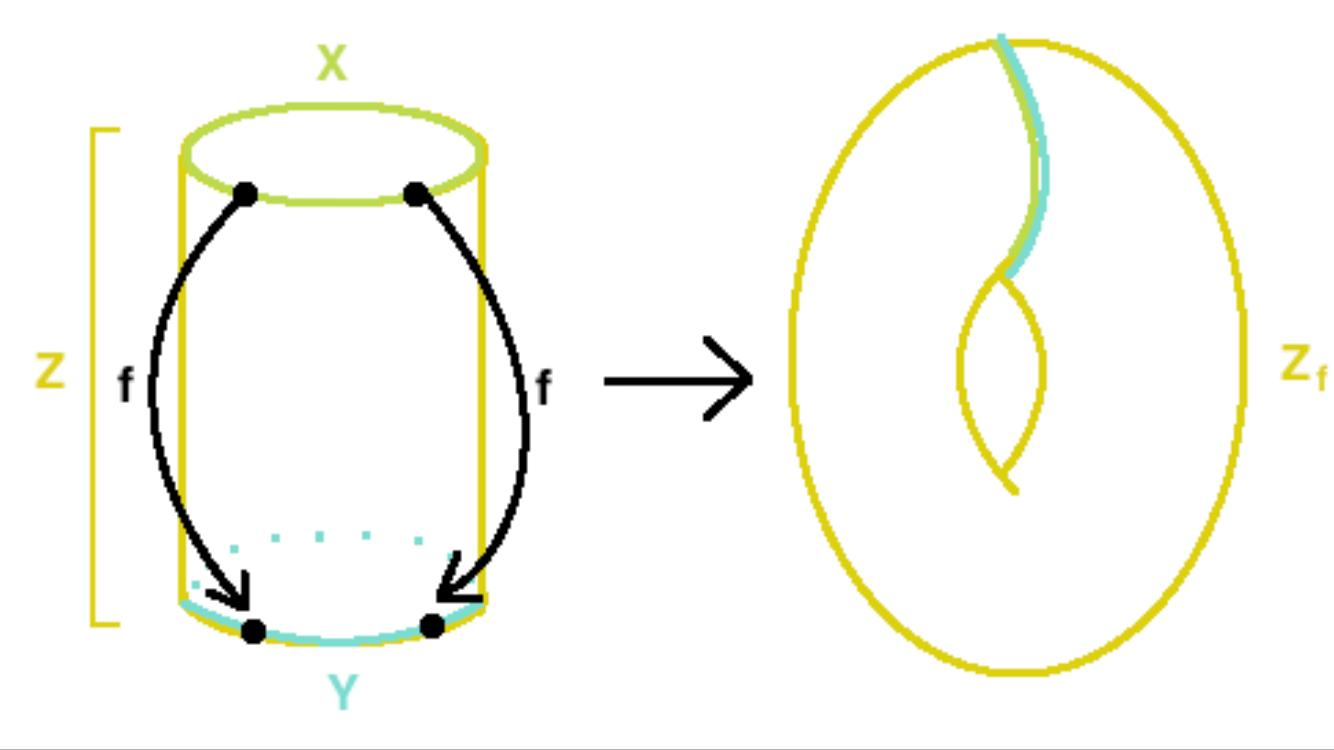
\includegraphics[scale = 0.3]{fotos_topo_1/gluinglemma2.jpeg}
\end{equation}

\begin{lema}
\label{lema:identificacionshomeomorf} Sigui $f:X\rightarrow Y$ una identificació. Aleshores $Y$ és homeomorf a $X/R_f$.
\end{lema}
\begin{proof}
Per definició de la relació d'equivalència tenim una aplicació de conjunts injectiva $\varphi:X/R_f\rightarrow Y$ tal que $f = \varphi\circ q$, on $q$ és l'aplicació de pas al quocient (\ref{def:pasalquocient}) $q:X\rightarrow X/R_f$. A més a més, com $f$ és exhaustiva, tenim que $\varphi$ és exhaustiva i, per tant, bijectiva. Com que $Y$ i $X/R_f$ tenen les topologies finals, per a un subconjunt $U$ de $Y$ tenim: $U$ és obert si, i només si $f^{-1}(U) = q^{-1}(\varphi^{-1}(U))$ és obert, i si i només si $\varphi^{-1}(U)$ és obert. Així doncs, $\varphi$ és un homeomorfisme.
\end{proof}

\begin{ej}
\label{ej:enganxamentihomeomorfisme} Sigui $X$ un espai topològic i sigui $A\subset X$ un subconjunt. Definim la relació d'equivalència
\begin{equation}
    \notag
    x R_A x\quad \text{per a tot}\quad x\in X,
\end{equation}
\begin{equation}
    \notag
    x R_A y\quad \text{per a tot}\quad x,y\in A
\end{equation}
Denotem per $X/A$ el conjunt $X/R_A$ amb la topologia final respecte de l'aplicació quocient (per tant, topologia quocient). Diem que hem identificat $A$ en un punt.

Per exemple, siguin $X = [0,1]$ i $A = \{0,1\}$. La relació d'equivalència $R_A$ coincideix amb $R_f$, on $f$ és l'aplicació $f:[0,1]\rightarrow S^1$, $f(x) = (\cos(2\pi x),\sin(2\pi x))$. Segons el lema, $X/A$ és homeomorf a $S^1$.
\end{ej}

\begin{ej}
\label{ej:espaienganxament} Considerem l'espai $Z = [0,3]$ i els subespais $X,Y\subset Z$ donats per $X = [0,1]$ i $Y = [2,3]$. Definim la funció $f:X\rightarrow Y$ per $f(x) = 3-x$. L'espai resultant $\mathcal{Z}_f$ pot ser representat com:
\begin{equation}
    \notag
    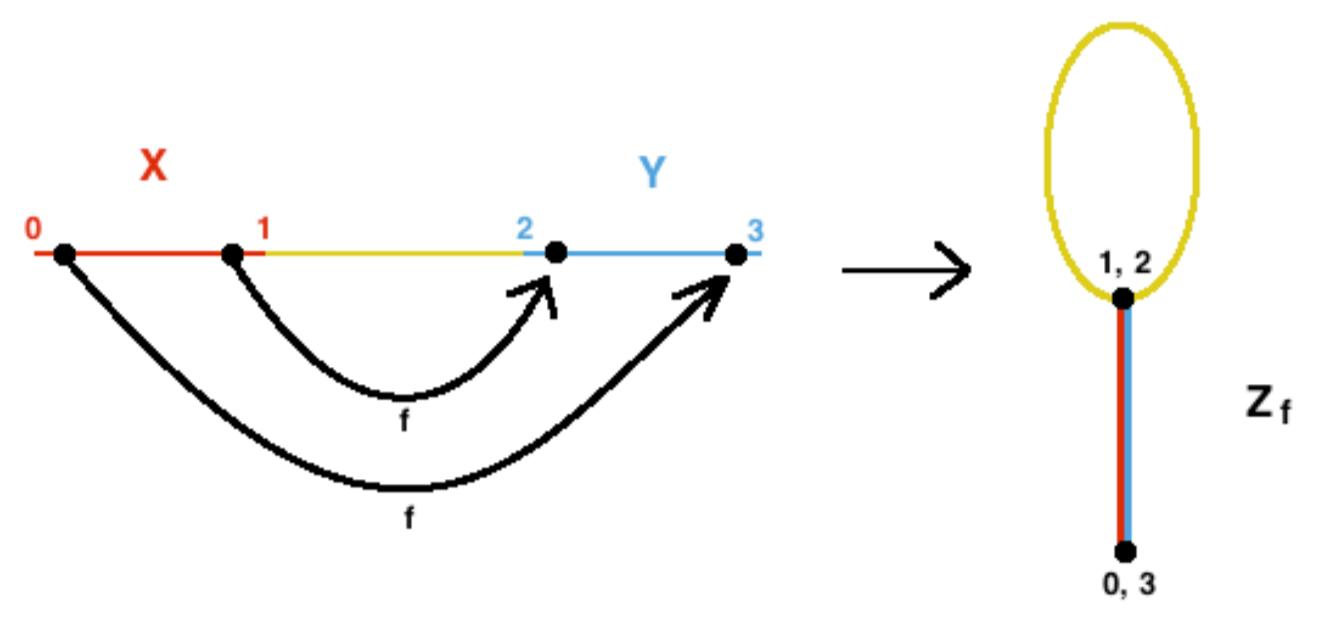
\includegraphics[scale = 0.3]{fotos_topo_1/gluinglemma3.jpeg}
\end{equation}
\end{ej}

\subsection{Enganxant espais topològics disjunts}

\begin{defi}
[Enganxament de dos espais topològics]\label{def:enganxamentdedosespaistopologics}\index{Enganxament de dos espais topològics} Siguin $X$ i $Y$ dos espais topològics disjunts. Sigui $A\subseteq X$ no buit i $f:A\rightarrow Y$ una aplicació tal que $f(A) = B$. Definim la relació d'equivalència $\sim$ a $X\cup Y$ d'aquesta forma:
\begin{equation}
    \notag
    x\sim y \Leftrightarrow \left\{
    \begin{array}{ll}
        f(x) = y \\
        \text{o bé}\\
        x = y
    \end{array}
    \right.
\end{equation}
És a dir, amb la relació $\sim$ associem punts que estan associats per $f$ així com els que estan associats per si mateixos. Les classes d'equivalència de $\sim$ són 
\begin{equation}
    \notag
    \{\{y\}\cup f^{-1}(y)\;:\;y\in B\},\quad \text{i els singletons}\quad \{\{y\}\;:\;y\in B\} .
\end{equation}
El resultat es diu \textit{enganxament de $X$ i $Y$ a partir de $f$} i es denota $(X\oplus Y)/\sim$ o també $X\cup_f Y$.
\end{defi}

\begin{equation}
    \notag
    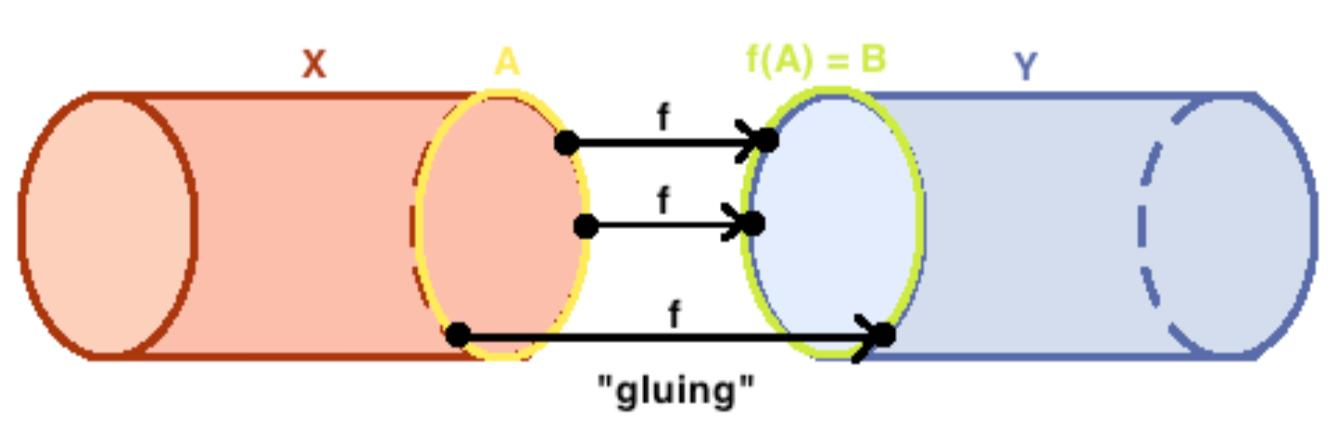
\includegraphics[scale = 0.3]{fotos_topo_1/gluinglemma4.jpeg}
\end{equation}

En termes més simples, considerem espais topològics disjunts $X$ i $Y$ i considerem un subconjunt $A$ de $X$. Sigui $f:A\rightarrow Y$ una funció on $f(A) = B$. Aleshores nosaltres enganxem els punts d'$A$ amb les seves respectives imatges per $f$ (que estan a $B\subseteq Y$ i també enganxem els punts que no siguin a $A$ amb ells mateixos.

\begin{ej}
\label{ej:enganxamentdedosespaistopologics} Un exemple molt simple és considerar els següents espais topològics disjunts: $X = [0,1]$ i $Y = [2,3]$, amb les topologies subespais de $\mathbb{R}$. Sigui $A = \{0.1\}$ i definim, per $x\in A$, la funció $f(x)$ com $f(0) = 2$ i $f(1) = 2$. Aleshores, enganxant els punts $0,1\in[0,1]$ amb les seves imatges (que és el 2) obtenim $(X\oplus Y)/\sim$.
\begin{equation}
    \notag
    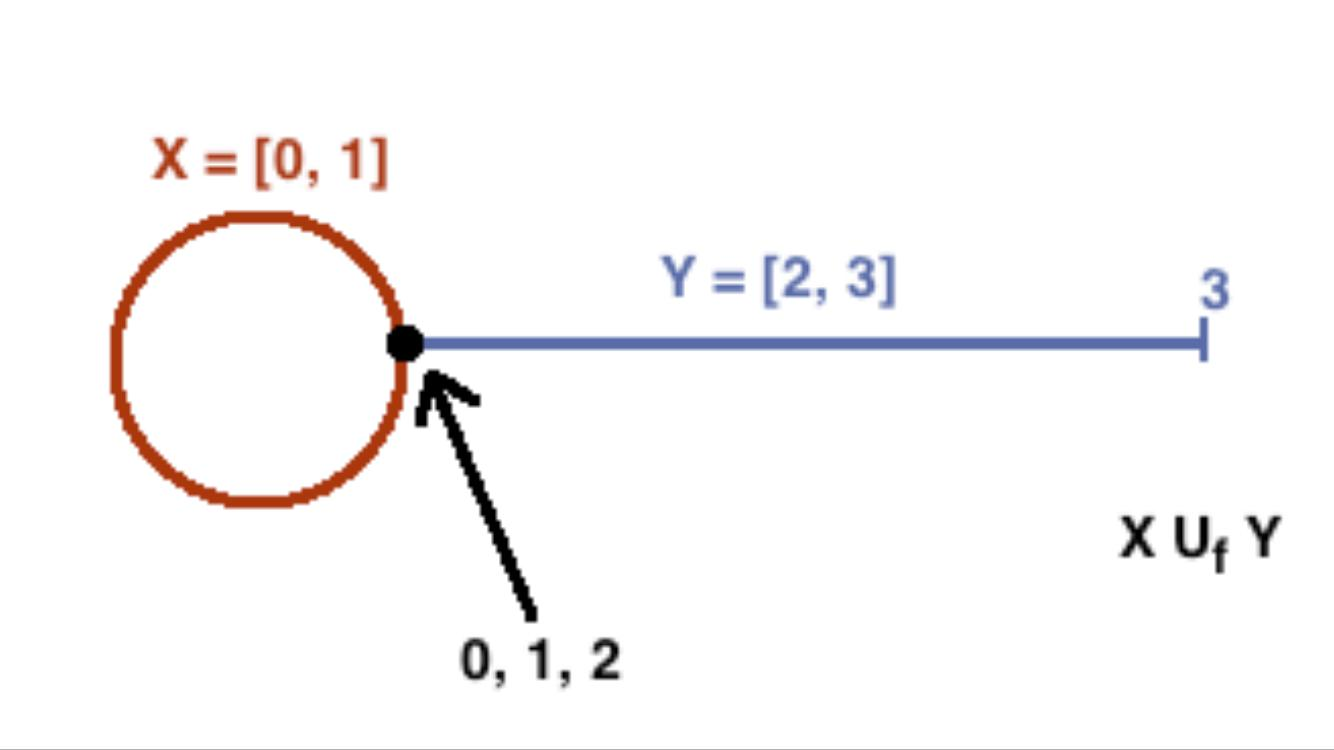
\includegraphics[scale = 0.3]{fotos_topo_1/gluinglemma5.jpeg}
\end{equation}
\end{ej}

\subsection{La construcció de la banda de Möbius}

Considerem el quadrat unitat $Z = [0.1]\times[0,1]$ en $\mathbb{R}^2$ i sigui $X = \{0\}\times[0,1]$ i $Y = \{1\}\times [0,1]$ com al dibuix:
\begin{equation}
    \notag
    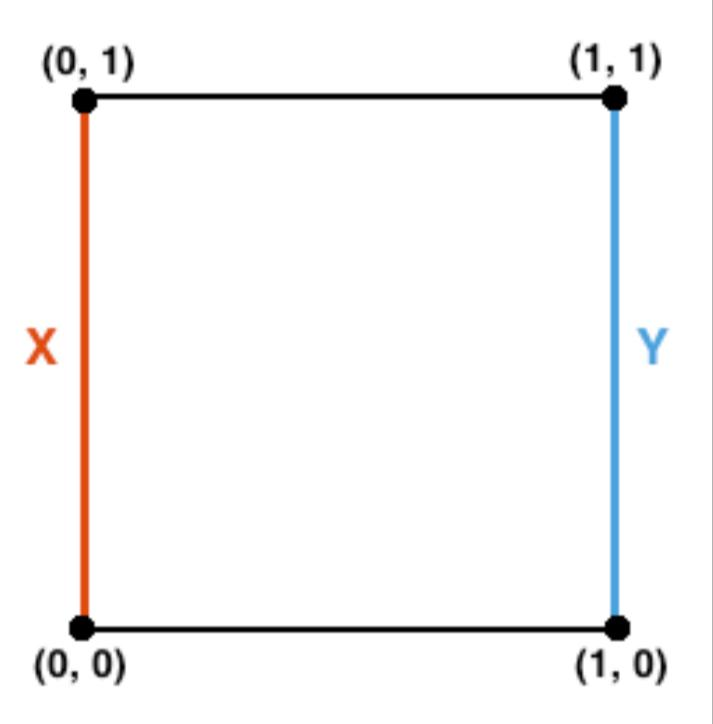
\includegraphics[scale = 0.3]{fotos_topo_1/gluinglemma6.jpeg}
\end{equation}
Definim la funció $f:X\rightarrow Y$ per $f(0,x) = (1,1-x)$.
\begin{equation}
    \notag
    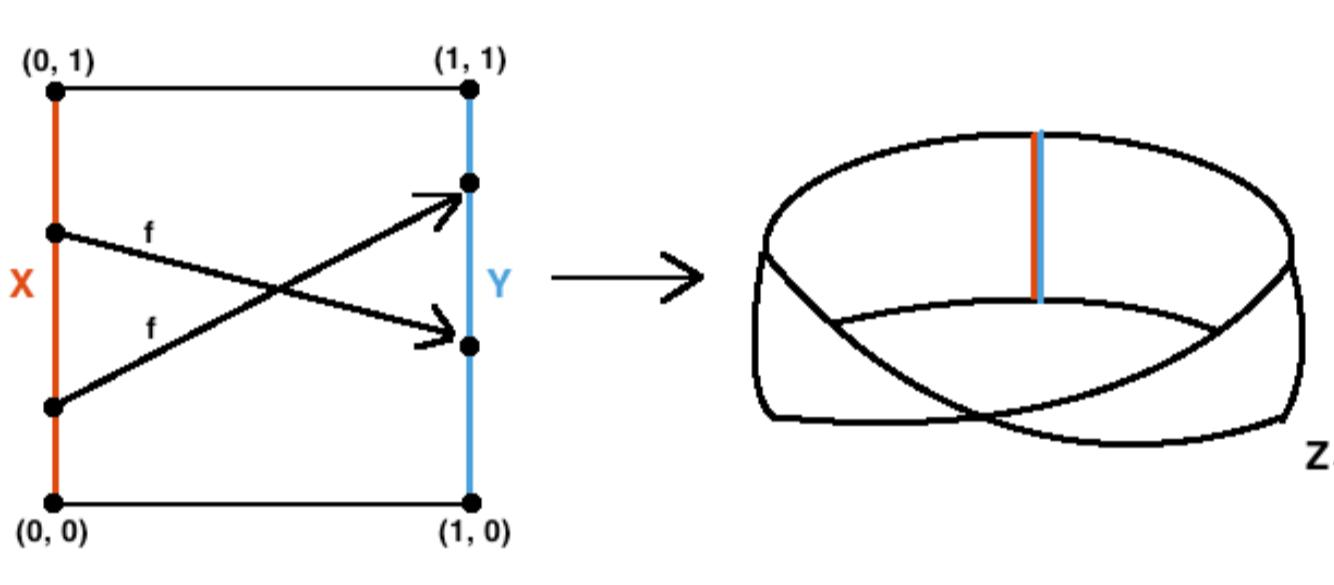
\includegraphics[scale = 0.3]{fotos_topo_1/gluinglemma7.jpeg}
\end{equation}
El resultant espai topològic $\mathcal{Z}_f$ és la coneguda banda de Möbius.

\subsection{La construcció del pla projectiu real}

Aquest apartat el copiaré de Wikipedia, ja que està bastant ben explicat.

La construcció d'aquest pla projectiu està basada en la Banda de Möbius: si es pogués enganxar la vora simple de la tira de Möbius en la direcció correcta, s'obtindria el pla projectiu (la qual cosa no és possible a l'espai tridimensional sense ue la superfície s'intersequi amb si mateixa). De manera equivalent, enganxar un disc al llarg del límit de la banda de Möbius da el pla projectiu.

Com que la banda de Möbius hem vist que es pot construir a partir d'un quadrat enganxant dos dels seus costats, el pla projectiu es pot presentar com un quadrat unitari $[0,1]\times[0,1]$ amb els seus costats identificats per les següents relacions d'equivalència:
\begin{equation}
    \notag
    (0,y)\sim (1,1-y),\qquad 0\leq y\leq 1
\end{equation}
i
\begin{equation}
    \notag
    (x,0)\sim(1-x,1),\qquad 0\leq x\leq 1
\end{equation}

\subsection{Altres construccions}

Veiem altres exemples d'aquest tipus:
\begin{enumerate}
    \item El cilindre $(0,1)\times S^1$.
    
    Com que $S^1$ és la identificació dels punts 0 i 1 en l'interval $[0,1]$ com ja es va veure, tenim que el cilindre també es pot descriure identificant en $X = [0,1]\times (0,1)$ els punts de la forma $(0,t)$ amb els de la forma $(1,t)$. Això està explicat en (\ref{ej:topologiaquocient1}) i en (\ref{ej:topologiaquocient2}). Observem que aquest cilindre és localment euclidià de dimensió 2, ja que un entorn d'un punt és la unió de dos semicercles
    \item El tor o torus $\mathbb{T}$.
    
    Ja vam veure a (\ref{ej:topologiaquocient2}) que el torus s'obtenia fent les identificacions que diu el dibuix. Vam veure també a (\ref{ej:tor}) que el tor era homeomorf a $S^1\times S^1$.
    \item El pla projectiu real $\mathbb{P}^2$. (alternativa)
    
    Aquest espai s'obté identificant a $S^2$ els punts antipodals. Sigui $H^+$ la semiesfera superior tancada. No és difícil provar que la restricció $H^+\rightarrow \mathbb{P}^2$ és també una identificació (aquest no és un fet general!). Utilitzant que $H^+$ i $X= I\times I$ són homeomorfs, aconseguim presentar el pla projectiu ral com l'espai obtingut identificant en el quadrat $X$ els punts de la frontera.
\end{enumerate}





\end{document}